\chapter{EXPERIMENT DESCRIPTION}
\label{sec:experiment_description}
\section{Experiment setup}

\begin{figure}[htbp]
    \centering
    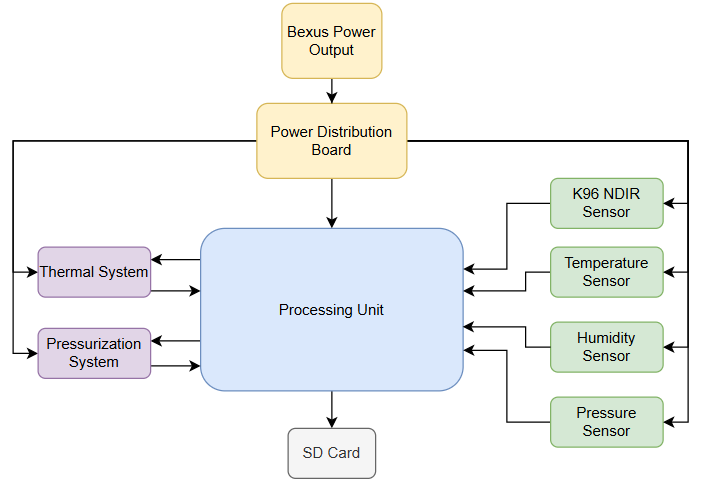
\includegraphics[width=0.8\textwidth]{0_images/figures/Mirage Block schematic.png}
    \caption{Experimental Setup}
    \label{fig:experimental_setup}
    
\end{figure}

The experiment will feature a NDIR sensor (K96), a pressurization system, a thermal system, ambient environment sensors and a processing unit. 
The pressurization system will include a pumping mechanism in order to increase the pressure and the amount of particles that can be measured. The air will be heated up and pumped into the measurement chamber with the K96 sensor inside together with temperature, pressure and humidity sensors. The gas will be exchanged continously to exchange the sample while maintaining the pressure of 3 bar. 
The K96 Sensor will communicate with the processing unit and the processing unit sends the measured digital data for storage to the SDHC card.
The pressure sensor,temperature sensor and humidity sensor communicate with the processing unit via digital interfaces (such as $I^2C$) to ensure that the pump and thermal control system are running with the right parameters to maintain room temperature conditions and a stable pressure of 3 bar. Unique addresses are used to identify each sensor's signal, allowing the processing unit to collect and organize data from all ambient sensors efficiently.

%%%%%%%%%%%%%%%%%%%%%%%%%%%%%%%%%%%%%%%%%%%%%%%%%%%%%%%%%%%%%%%%%%%%%%%%%%%%%%%
\section{Experiment Interfaces}

%%%%%%%%%%%%%%%%%%%%%%%%%%%%%%%%%%%%%%%%%%%%%%%%%%%%%%%%%%%%%%%%%%%%%%%%%%%%%%%
\subsection{Mechanical Interface}\label{mechanical_interface}

The \gls{mirage} enclosure is mechanically attached to the ESCARGO gondola structure via four mounting points located on its bottom plate. These four connection points interface with two parallel 45 $\times$ 45 mm Bosch aluminium T-slot profiles using M6 T-bolts, M6 rubber spacers, and M6 flange nuts. The parallel profiles are then mounted to the ESCARGO gondola structure using standard Rexroth M6 brackets, M6 T-bolts, and M6 flange nuts. This configuration facilitates installation without necessitating structural modifications to the ESCARGO frame, ensuring full compatibility with the standard mounting interface.

To reduce vibration transmission, temperature transfer and accommodate minor alignment tolerances during installation, rubber spacers are installed between the enclosure and the mounting brackets.

The mounting configuration provides a rigid mechanical interface between the experiment enclosure and the ESCARGO frame, ensuring structural redundancy and compliance with the standard ESCARGO mechanical interface requirements.

\begin{table}[htbp]
\centering
\begin{tabular}{lcl}
\toprule
\textbf{Item} & \textbf{Quantity} & \textbf{Specification} \\
\midrule
L-bracket & 4 & Bosch Rexroth aluminium M6 bracket \\
T-Bolt & 12 & M6 $\times$ 25 mm \\
Flange nut & 12 & M6 \\
Rubber Spacer/Damper & 4 & M6 \\
\bottomrule
\end{tabular}
\caption{Mounting hardware components}
\label{tab:mounting_hardware}
\end{table}

\begin{figure}[H]
    \centering
    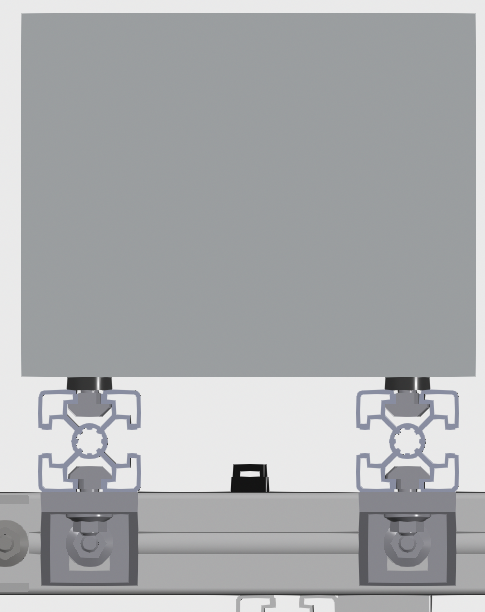
\includegraphics[width=0.45\textwidth]{0_images/figures/mouting.png}
    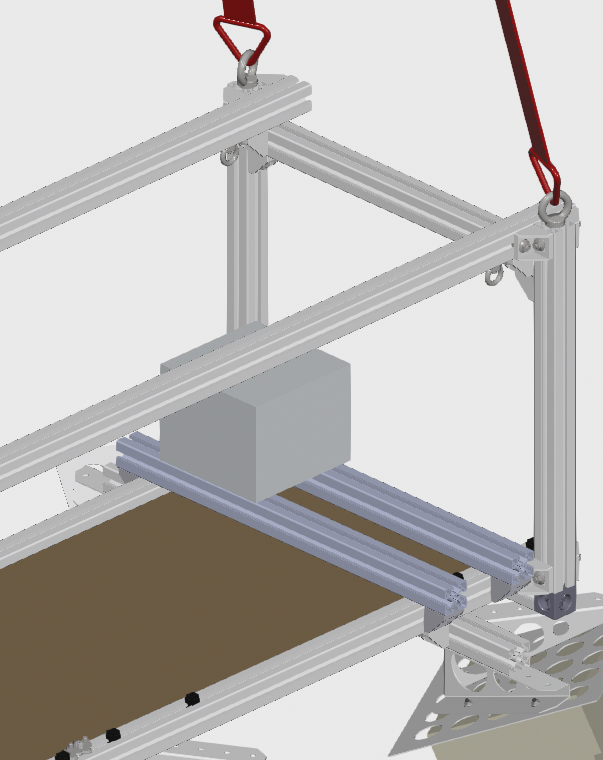
\includegraphics[width=0.45\textwidth]{0_images/figures/render3.png}
    \caption{CAD images of the mechanical interface.}
    \label{fig:example_image}
    
\end{figure}
%%%%%%%%%%%%%%%%%%%%%%%%%%%%%%%%%%%%%%%%%%%%%%%%%%%%%%%%%%%%%%%%%%%%%%%%%%%%%%%
\subsection{Electrical Interface}\label{electrical_interface}

The electrical interface to the Bexus power unit consists of the MIL-C 26482P series 1 connector, as provided by the user manual. Using pin A and B, the supply voltage from the SAFT MP176065 battery pack will be fed to the power distribution board.
The connector to the E-Link of the gondola will be an Amphenol RJF21B and the RJ45 connector will be employed for communication with a RJ45 plug on the MCU PCB.

Since the Bexus power supply is 28.8V two LM2596HVS step-down voltage regulators will be used on the power distribution board. For the MCU and K96 sensor 8V will be used, the pressurization system operates at 24V, the thermal system at 12V and 3.3V for the sensors. The estimated average current draw from the BEXUS battery is 0.8A and the average power consumption is 23.11W. The total power consumption from BEXUS power unit is 138.67Wh as listed in section 4.7 and the peak current draw is 2.26A. For protecting the BEXUS batteries and other experiments a pre-charge circuit will be implemented in order to limit the currents of the pressurization system and an LC filter to deal with the EMI and switching frequencies of DC/DC converters. Distributed single point ground will be implemented.


%%%%%%%%%%%%%%%%%%%%%%%%%%%%%%%%%%%%%%%%%%%%%%%%%%%%%%%%%%%%%%%%%%%%%%%%%%%%%%%
\subsection{Thermal}\label{thermal}
As outlined in \sref{sec: thermal design}, the thermal behaviour of the experiment will be controlled via heating elements and insulation. To avoid thermal coupling to ESCARGO, rubber bumpers between the experiment and the gondola will be used.
The thermal coupling will be further tested when the experiment is assembled. The air inlet and outlet for the air samples to be measured will be directed away from the vehicle and should not heat or cool the vehicle.

%%%%%%%%%%%%%%%%%%%%%%%%%%%%%%%%%%%%%%%%%%%%%%%%%%%%%%%%%%%%%%%%%%%%%%%%%%%%%%%
\section{Experiment Components}

\begin{table}[H]
\centering
\caption{Experiment summary table}
\label{tab:experiment_summary}
\begin{tabular}{L{6cm}L{6cm}}
\toprule
Experiment mass (in kg): & $\sim$4.0 \\
Experiment dimensions (in m): & 0.20x0.20x0.15\\
Experiment expected \gls{cog} position: & Distance from geometric centre: x=4mm y=23mm z=22mm \\
\bottomrule
\end{tabular}
\end{table}

\begin{table}[H]
\centering
\caption{Electrical components}
\label{tab:electrical_components}
\begin{tabular}{p{4cm}p{4cm}ll}
\hline
\textbf{Component} & \textbf{Dimensions (mm)} & \textbf{Mass (g)} & \textbf{Quantity}\\
\hline
Vacuum pump & 119$\times$44$\times$73 & 294 & 2 \\
Compressor & 130$\times$60$\times$85 & 445 & 1 \\
Arduino Mega & 54$\times$102$\times$15 & 37 & 1\\
K96 & 42.26$\times$33.9$\times$26.04 & 300 & 1 \\
MS5607 & 3.0$\times$5.0$\times$0.95 & <1 & 1\\
SHT45 & 1.5$\times$1.5$\times$0.5 & <1 & 4 \\
LM2596HVS-ADJ & 10.1$\times$9.0$\times$4.5 & 1.59 & 3 \\
\gls{pcb} & TBD & TBD & 1 \\
Thermal system & TBD & TBD &  \\
\hline
Total & & 1079.59 & \\
\hline
\end{tabular}
\end{table}

%%%%%%%%%%%%%%%%%%%%%%%%%%%%%%%%%%%%%%%%%%%%%%%%%%%%%%%%%%%%%%%%%%%%%%%%%%%%%%%
\section{Mechanical Design}\label{mechanical_design}

The mechanical design of the \gls{mirage} experiment focuses on a compact enclosure housing a pressurized measurement chamber, a multi-stage pump system, supporting electronics, and a heating system. \gls{mirage} is designed to fit within the ESCARGO gondola structure while maintaining structural integrity and ensuring safe operation under the environmental conditions expected during the mission.

\begin{figure}[htbp]
    \centering
    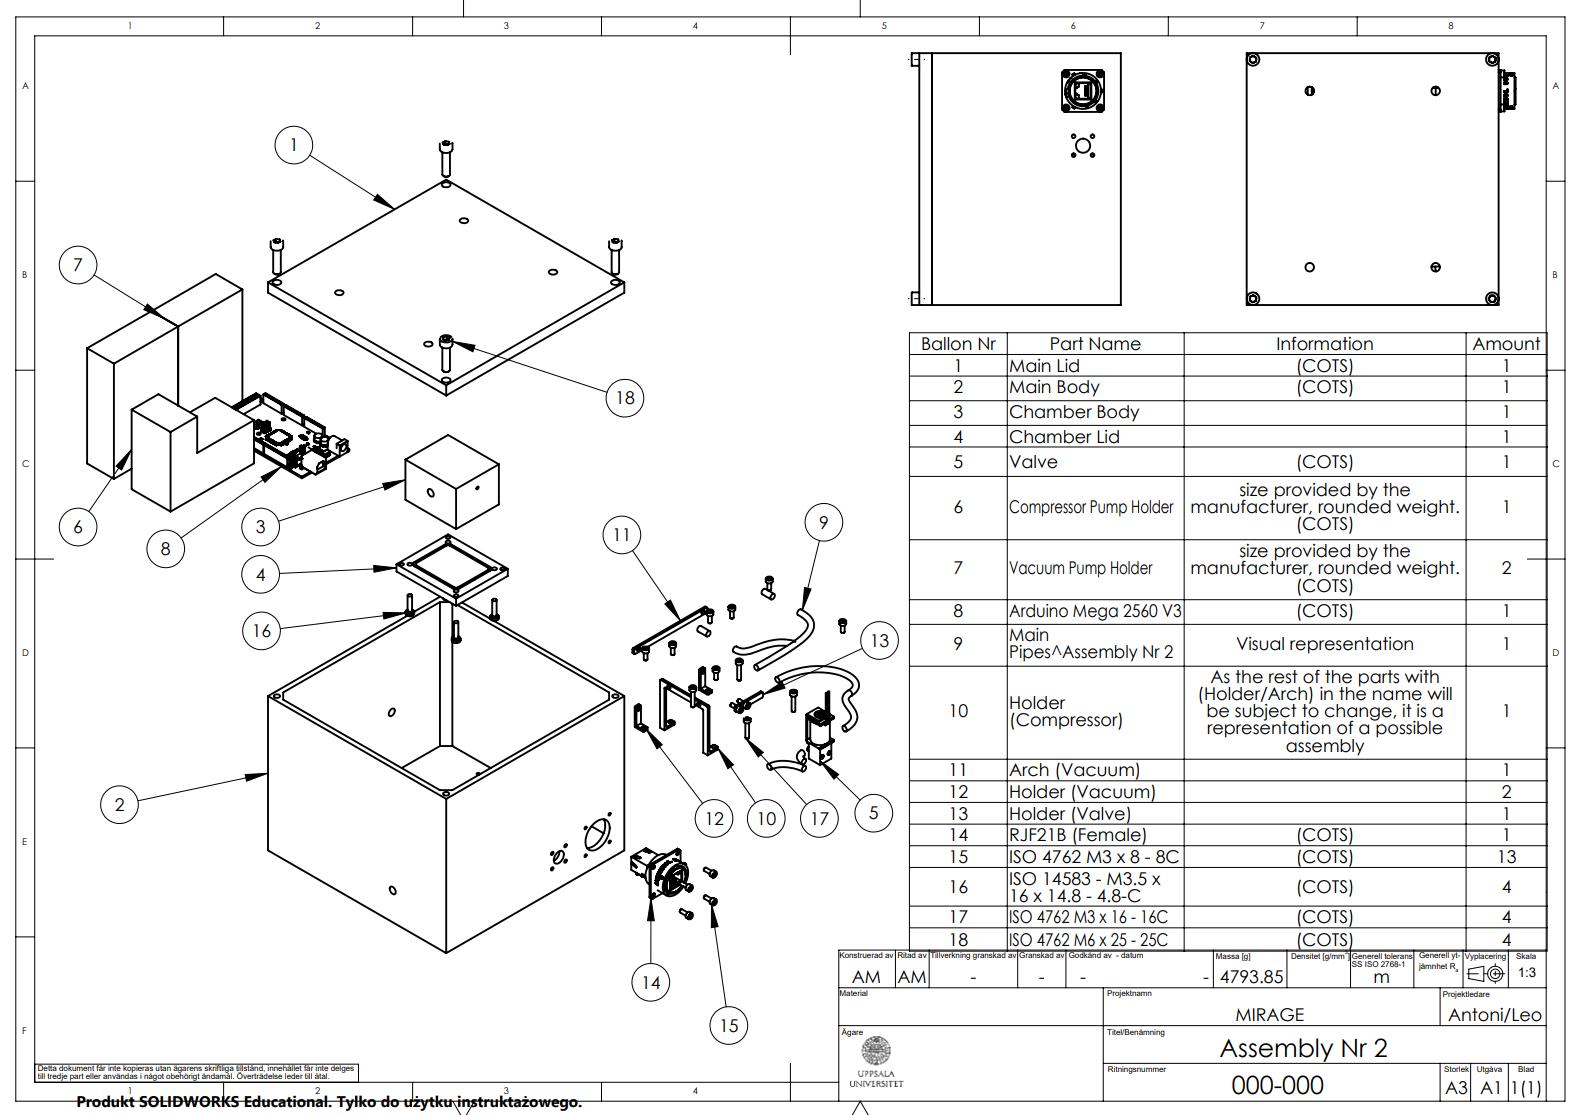
\includegraphics[width=0.8\textwidth]{0_images/figures/tech_drawing.png}
    \caption{Technical drawing of the system as a whole.}
    \label{fig:tech_drawing}
    
\end{figure}

\subsection{Experiment Enclosure}

The experiment is housed in a \gls{cots} aluminium enclosure with external dimensions of $200\times 200\times 150$ mm and a wall thickness of expected 2 mm. The enclosure provides mechanical protection for all internal components and acts as the primary structural body of the experiment. A \gls{cots} enclosure was selected to reduce manufacturing complexity, minimize cost, and provide a robust structural housing with well-characterized mechanical properties.
The enclosure is directly mounted to the ESCARGO frame as described in \sref{mechanical_interface}. Internally, the enclosure accommodates the pressure chamber, two diaphragm vacuum pumps, one piston compressor, a passive outflow hole, shutter valve, tubing, and electronic control hardware. The enclosure also includes two dedicated holes for air inlet and one for outlet, as well as electrical feedthroughs required for connecting to the BEXUS power and E-link system.

\begin{figure}[htbp]
    \centering
    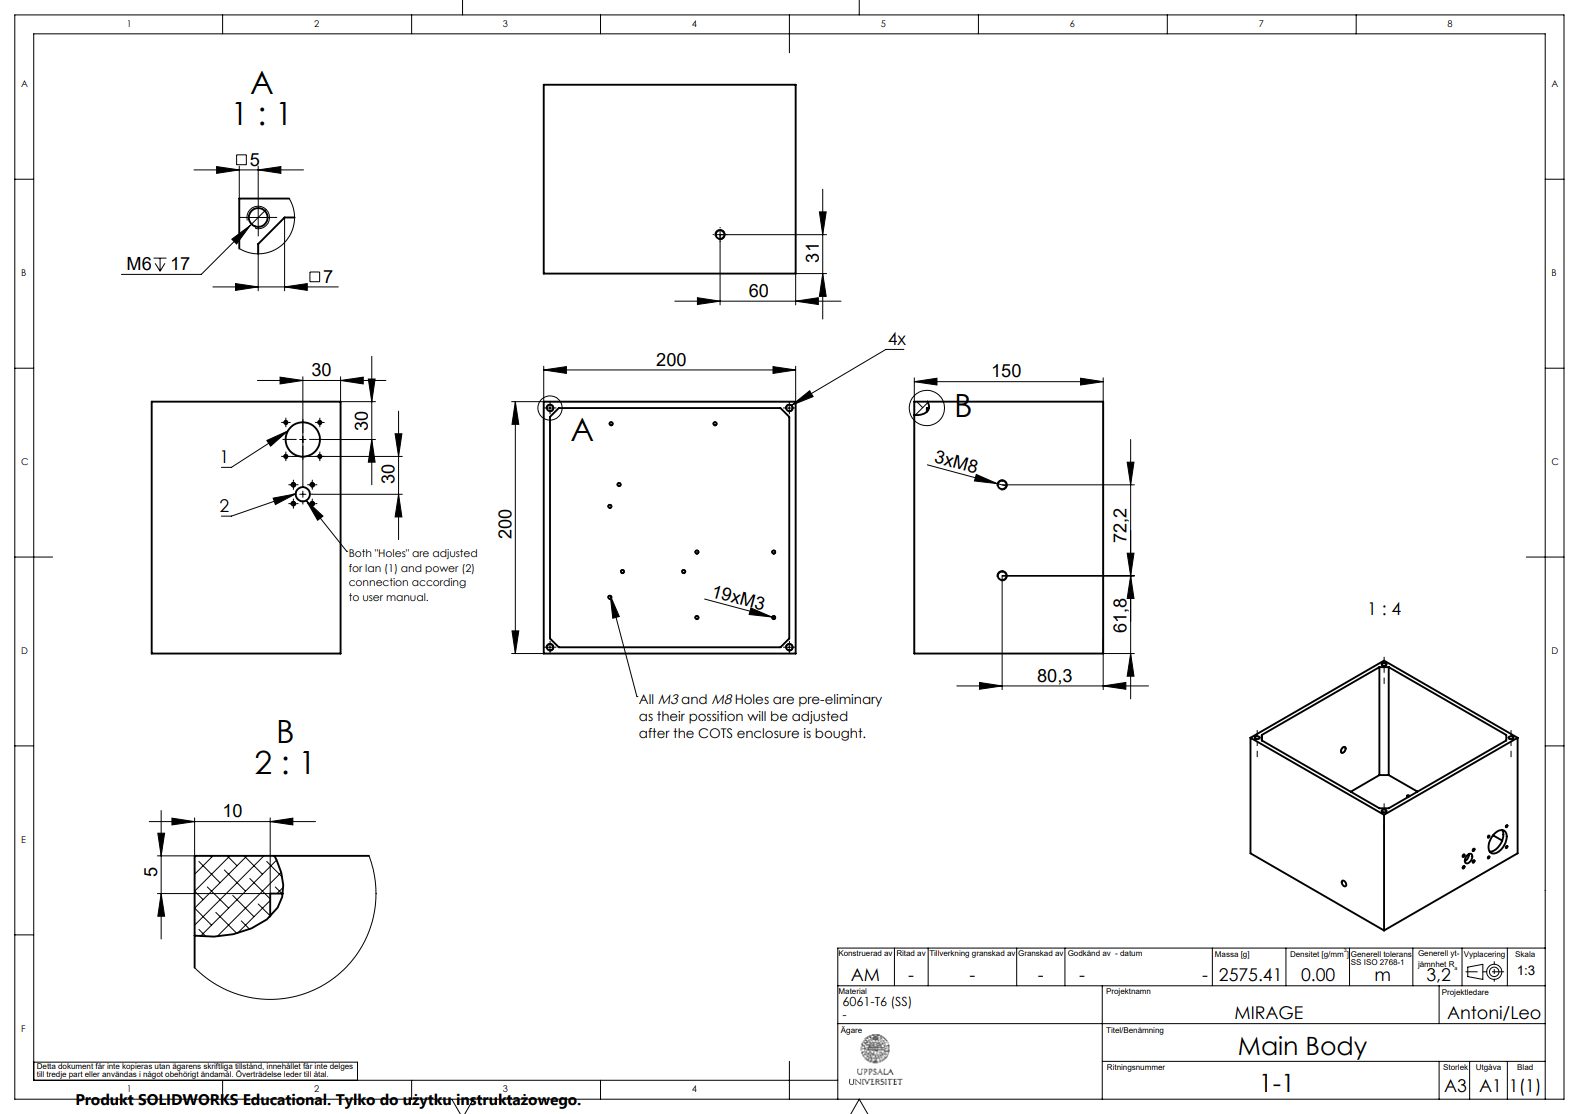
\includegraphics[width=0.45\textwidth]{0_images/figures/tech_drawing_3.png}
    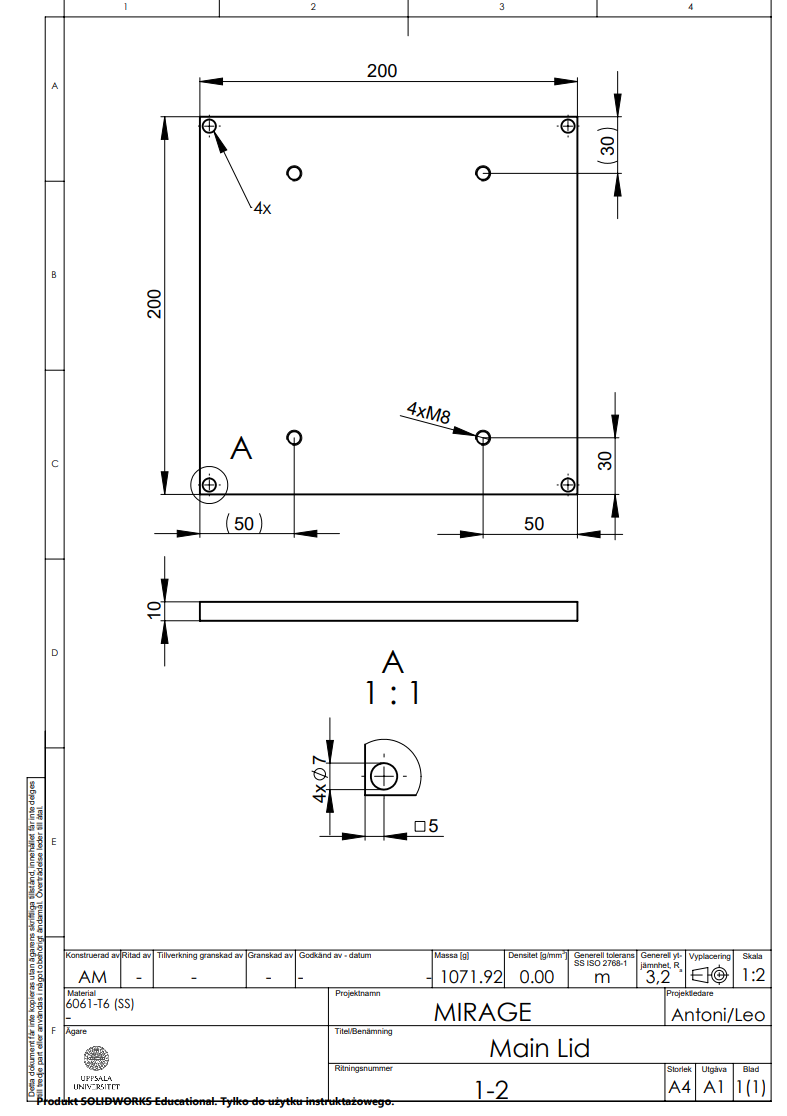
\includegraphics[width=0.45\textwidth]{0_images/figures/tech_drawing_5.png}
    \caption{Technical drawings of experiment enclosure. Drawings are representative and the thickness of both “Main Body” and “Main Lid” will be reduced to 2mm by buying COTS parts.}
    \label{fig:enclosure}
\end{figure}

\subsection{Internal Layout}

The internal layout of the \gls{mirage} experiment is arranged to maintain a compact configuration and minimize the length of the airflow path between the pressurized chamber and the compressor.
Electronic control hardware is mounted along the inner bottom of the enclosure, providing physical isolation between electrical components and the pressurized air system.
This configuration ensures efficient airflow through the chamber while maintaining accessibility for integration and servicing.

\begin{figure}[htbp]
    \centering
    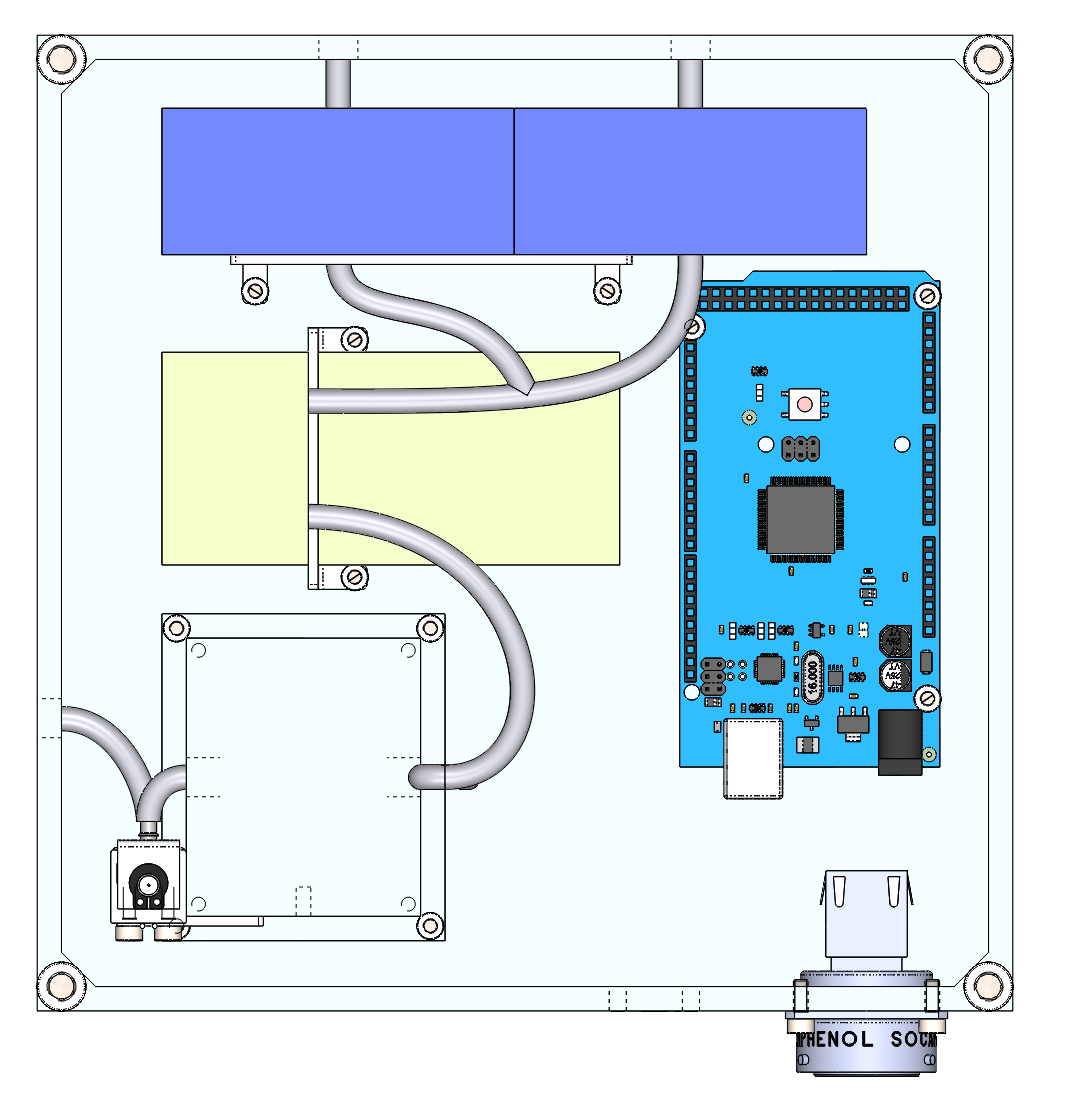
\includegraphics[width=0.8\textwidth]{0_images/figures/tech_drawing_6.png}
    \caption{Drawing of the internal layout.}
    \label{fig:int_layout}
    
\end{figure}

\subsection{Pressurized Measurement Chamber}

The core element of the experiment is a small pressurized chamber that houses the K96 sensor used for the measurements. The chamber has internal dimensions of approximately $38 \times 33 \times 45$ mm and a wall thickness of 7 mm. It will be machined from aluminium by the \gls{mirage} team at Uppsala University.

The chamber is sealed using a copper gasket to ensure reliable sealing under elevated pressure conditions and temperature changes. Copper gaskets were selected due to their ability to provide a robust metal-to-metal seal capable of maintaining integrity at high pressure differentials.

The chamber is designed to minimize internal volume while providing sufficient space for the sensor and the necessary airflow path. Reducing the internal volume proportionally lowers the airflow rate required to exchange the chamber atmosphere, which improves the overall performance of the experiment.

\begin{figure}[htbp]
    \centering
    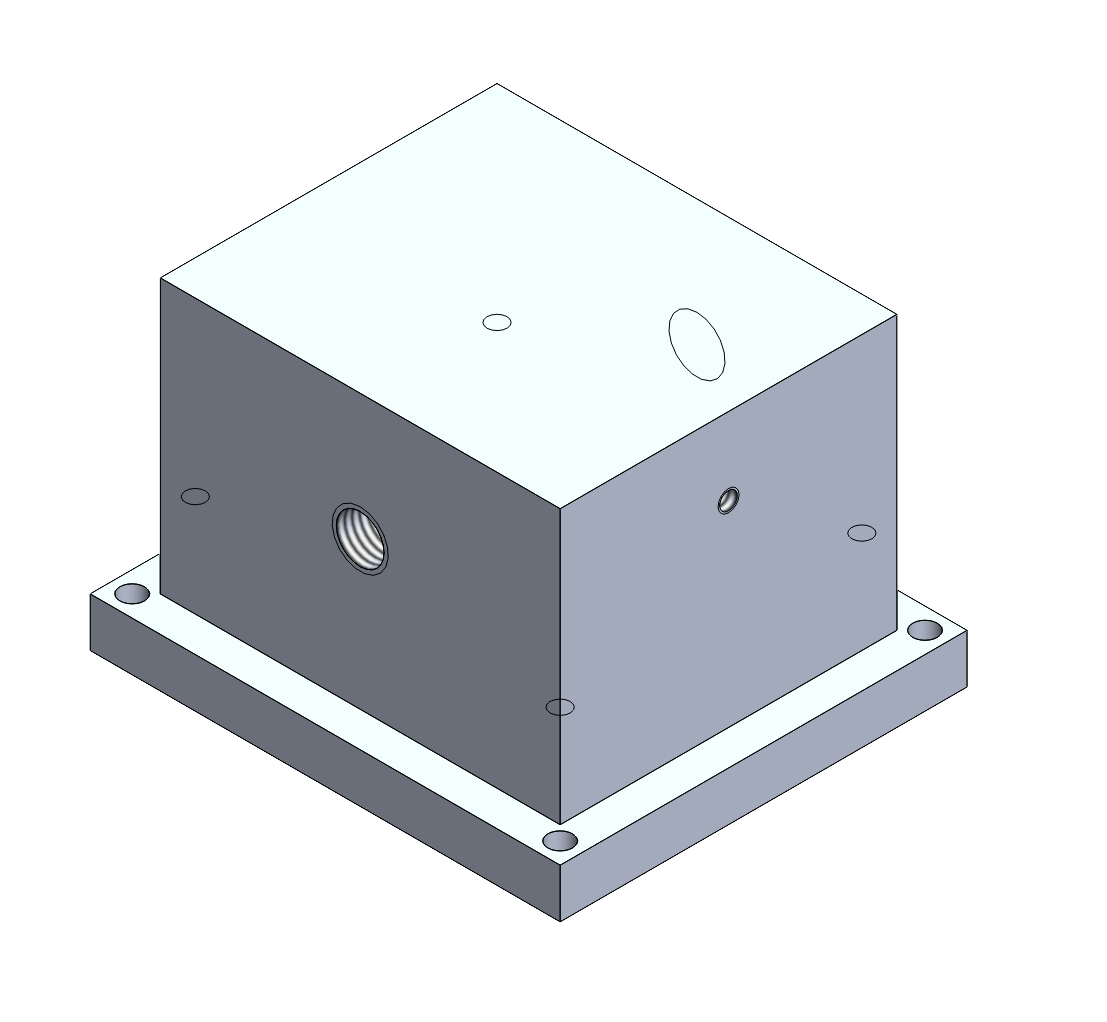
\includegraphics[width=0.45\textwidth]{0_images/figures/render2.png}
    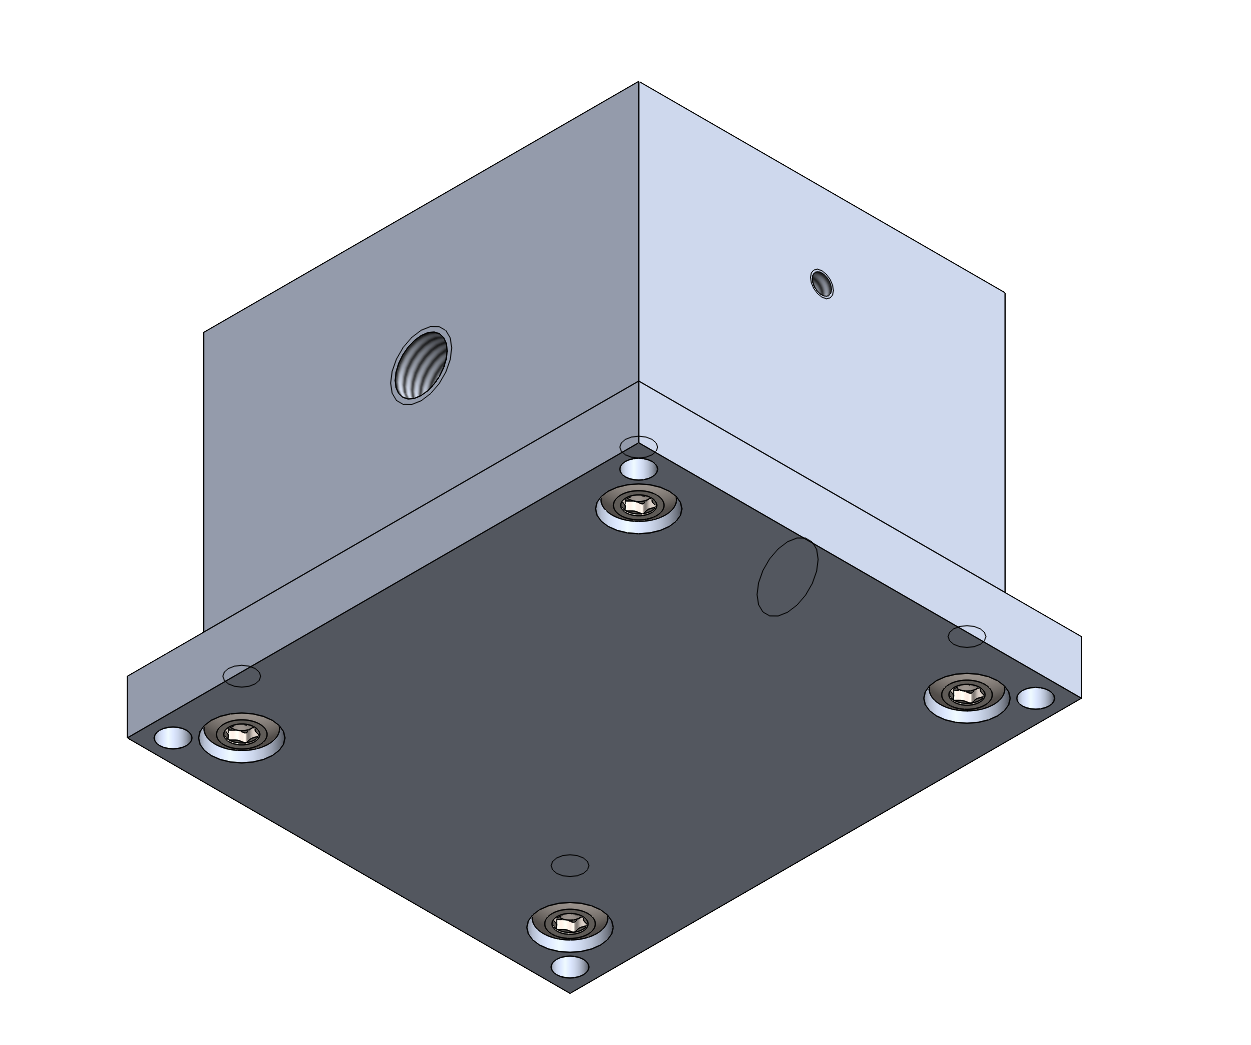
\includegraphics[width=0.45\textwidth]{0_images/figures/render1.png}
    \caption{Renders of the pressurized chamber.}
    \label{fig:pressure_render}
\end{figure}

\begin{figure}[htbp]
    \centering
    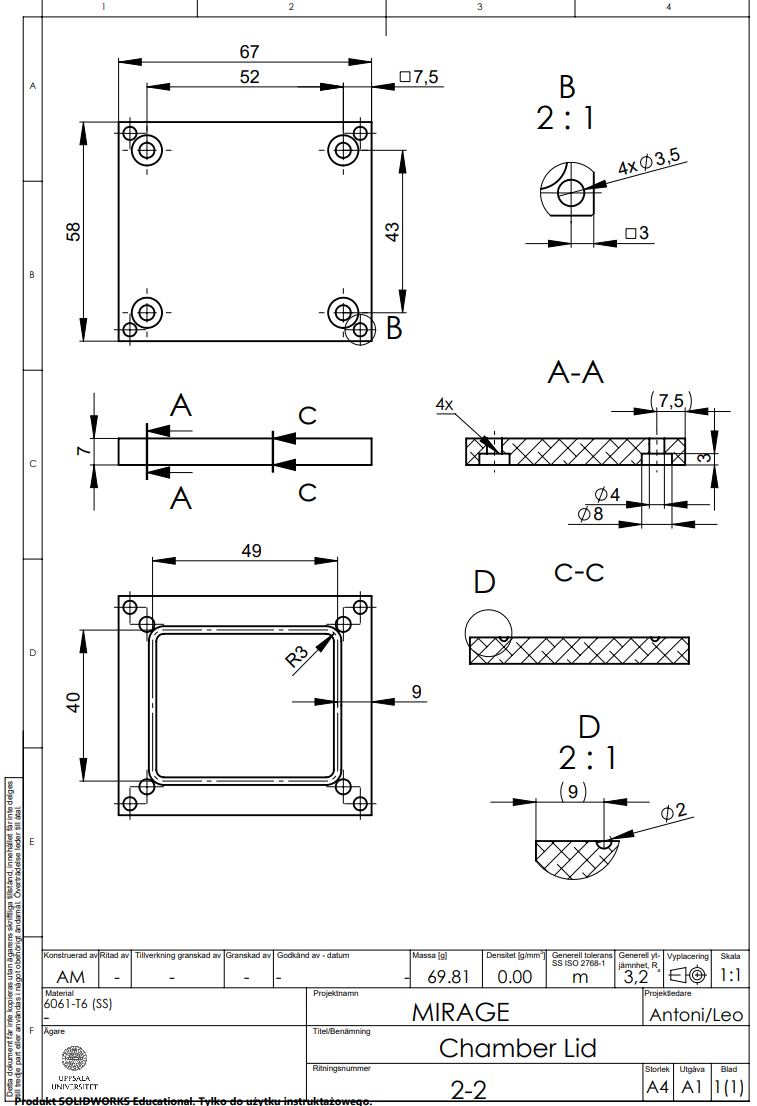
\includegraphics[width=0.45\textwidth]{0_images/figures/tech_drawing_2.png}
    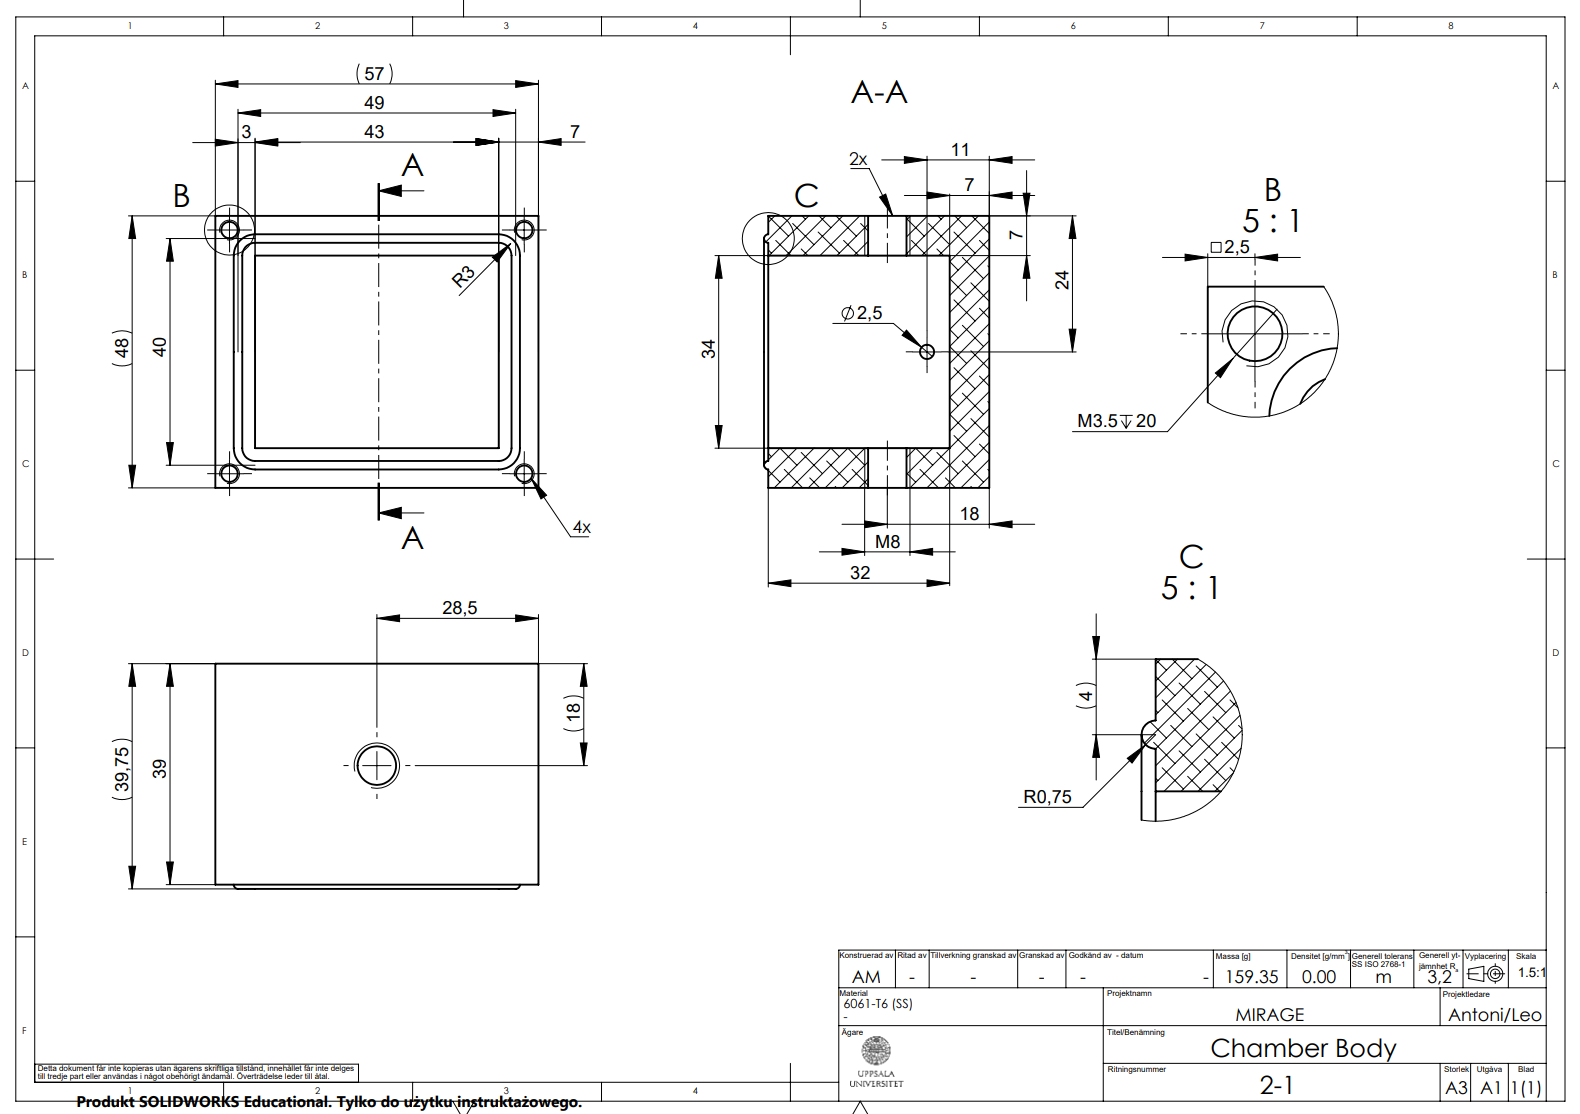
\includegraphics[width=0.45\textwidth]{0_images/figures/tech_drawing_4.png}
    \caption{Technical drawings of the pressurized chamber.}
    \label{fig:pressure_drawing}
\end{figure}

\subsection{Pump System Architecture}\label{sec: pump system arch}

The \gls{mirage} experiment utilizes a multi-stage air circulation system to maintain a controlled internal pressure while ensuring a continuous exchange of air within the measurement chamber.

\textbf{System Operation:}

\begin{enumerate}
    \item Pre-heating: Ambient intake air is pre-heated before entering the vacuum stage to prevent condensation or freezing within the system components.
    \item Vacuum Stage: Two diaphragm vacuum pumps operate continuously from launch up to an altitude of 22 km. These pumps supply the secondary stage with air at approximately atmospheric pressure ($\approx$ 1 bar). Since the volumetric flow rate decreases with decreasing intake pressure, the pumps will operate at higher settings at higher altitudes.

    \item Intercooling: To manage thermal loads generated by compression, the tubing connecting the vacuum pumps to the piston compressor serves as a passive intercooler.
    \item Compression Stage: A piston compressor increases the airflow pressure to a maximum of 3 bar before it enters the measurement chamber.
    \item Pressure Regulation: The internal chamber pressure is maintained by a passive outflow valve equipped with a shutter mechanism. This valve regulates the exhaust flow rate to the external environment.
    \item Monitoring: Integrated pressure and temperature sensors are situated within the tubing between compression stages to provide real-time performance data and ensure stable operation.
\end{enumerate}

%% ADD FIGURE %%

\textbf{Compressor Design Considerations:} Two primary design methodologies are being evaluated for the compression stage:

\begin{enumerate}
    \item Continuous Low-Flow Operation: Utilizing a compressor capable of maintaining a continuous, very low flow rate to match the chamber's exchange requirements.
    \item Intermittent Buffered Operation: Utilizing a higher flow rate compressor operated in duty cycles. This configuration requires a 1 bar buffer tank between pressurisation stages to accumulate air from the vacuum stage. The compressor activates to deplete the tank and deactivates once the tank pressure reaches a lower threshold.
\end{enumerate}

The nominal operating pressure inside the chamber is expected to reach approximately 3 bar above perfect vacuum. At float altitude, the external ambient pressure may decrease to approximately 10 mbar, resulting in a pressure differential of approximately 3 bar across the chamber walls. This pressure differential is accounted for in the structural design of the chamber.

The pressure between the vacuum pumps and the compressor is expected to remain close to atmospheric pressure ($\approx$ 1 bar) during normal operation in order to match expected compressor efficiency.

Temperature conditions at float altitude will require the implementation of pre-heating of the intake air before the vacuum stage to prevent condensation or freezing within the system. Additionally, pressure sensors will be placed between compression stages to monitor system performance and ensure stable pressure control during operation.

% \subsection{In-line Sensing and Environmental Monitoring}

% To ensure the operational integrity of the gas handling system and to facilitate real-time performance analysis, the \gls{mirage} experiment incorporates an integrated sensing suite within the tube circuit. This monitoring architecture is essential for validating the state of the air as it transitions through the various compression and thermal management stages.

% \begin{enumerate}
%     \item Pressure Sensing: High-precision pressure sensors are situated within the tubing between the diaphragm vacuum pumps and the piston compressor. These sensors monitor the inter-stage pressure to ensure that the vacuum pumps, operating continuously up to 22 km, maintain the required 1 bar supply pressure for the compressor.
%     \item Temperature Sensing: Thermal sensors are embedded directly into the flow path to monitor the effectiveness of the pre-heating and intercooling mechanisms. Monitoring the air temperature post-heating is critical to verify that the intake air has reached a safe threshold before entering the pump heads and K96 sensor chamber, thereby preventing damage from cold or heat
% \end{enumerate}

\subsection{Pump and Fluid Handling Technologies}

Small gas circulation and sampling systems used in atmospheric sensing instruments typically rely on compact electrically driven pumps to move air through measurement chambers and sensors. Several pump technologies are commonly used in portable gas analysis systems, including diaphragm pumps, piston compressors, rotary vane pumps, and scroll pumps. Each technology offers different advantages in terms of pressure capability, size, reliability, and maintenance requirements.

Diaphragm pumps are widely used in environmental monitoring and portable gas sampling instruments. These pumps operate by oscillating a flexible diaphragm using an electric motor, creating alternating suction and compression cycles. Because the gas is hermetically separated the mechanical drive components by the diaphragm, diaphragm pumps operate oil-free and are resistant to contamination. This makes them particularly suitable for experiments involving sensitive sensors or atmospheric gas sampling. Furthermore, diaphragm pumps are compact, lightweight, and tolerant of condensation in the airflow, which is expected in the \gls{mirage} experiment due to low external temperatures at float altitude.

Piston compressors are commonly used when higher pressures are required. These pumps use a reciprocating piston to compress air within a cylinder, allowing significantly higher pressure ratios than typical diaphragm pumps. However, piston compressors generally contain more moving mechanical parts and may be more sensitive to contamination or thermal effects. For this reason, piston compressors are often used in series with diaphragm pumps in small air circulation systems, where the diaphragm pumps provide initial airflow and the compressor increases the pressure to the required level.

Other pump technologies, such as rotary vane pumps and scroll pumps, are frequently used in laboratory vacuum systems. While these technologies can achieve significantly lower pressures and higher pumping speeds, they typically require lubrication, larger mechanical assemblies, and higher power consumption. Due to these characteristics, they are generally unsuitable for compact balloon payload experiments such as \gls{mirage}, where mass, power consumption, and system simplicity are critical design constraints.

Based on this comparison, diaphragm pumps were selected as the primary airflow drivers in the \gls{mirage} experiment due to their oil-free operation, compact size, reliability, and resistance to condensation. A piston compressor is used downstream of the diaphragm pumps to achieve the required pressurization of the measurement chamber.

\subsection{Tubing and Flow Control Components}

Gas flow regulation in compact atmospheric sensing instruments is traditionally achieved through the use of miniature solenoid or needle valves. Solenoid valves are often preferred for their rapid response times and ability to provide high-precision, electronically controlled flow regulation within automated systems.
However, for the \gls{mirage} experiment, the design has been optimized to utilize a passive outflow valve equipped with a mechanical shutter. This shift to a passive regulation system is engineered to maintain the required internal chamber pressure of approximately 3 bar by modulating the exhaust flow rate (hole size) based on the pressure differential encountered during the flight profile. In addition the usage of a shutter-based passive mechanism rather than an active solenoid, the system achieves greater mechanical simplicity and safety if the ballon would fall into the water.
The final selection of the hole and the shutter's mechanical properties is based on ensuring a stable airflow path that accommodates the continuous operation of the upstream diaphragm pumps up to the 22 km altitude threshold.

\subsection{Tubing and Fluid Connections}

The airflow between the pumps, compressor, and pressurized measurement chamber is transported through flexible tubing. In compact gas circulation systems, tubing connections are typically achieved using barbed fittings, compression fittings, or push-to-connect pneumatic fittings.

Barbed fittings are commonly used with flexible tubing materials such as silicone or polyurethane, where the tubing is pressed onto the fitting and secured through friction or hose clamps. Compression fittings provide a more robust and leak-tight connection and are frequently used in higher-pressure gas systems. Push-to-connect fittings are widely used in pneumatic systems due to their ease of installation and reliable sealing.

For the \gls{mirage} experiment, the tubing connections will be selected to ensure leak-tight operation at pressures up to approximately 3 bar while maintaining compatibility with the chosen tubing material and the compact geometry of the experimental setup. Particular attention will be given to minimizing leakage and dead volumes in the system to maintain stable pressure control and reliable airflow through the measurement chamber.

In alignment with the experiment's thermal management requirements, the intake tube lines will be integrated with high-conductivity copper windings to facilitate efficient heat transfer between the enclosure and the vacuum pump interface. This thermal exchange mechanism is designed to rapidly elevate the temperature of the intake air, ensuring the fluid stream remains within the pump's safe operational range. This will also be the case between compressor and the chamber as the heat created by compression could affect the quality of the study. This proactively mitigates the risk of mechanical failure or structural damage to the diaphragm components caused by the extreme low-temperature environment encountered during the ascent to 22 km and high temperatures after compression.

\subsection{Pumps}

The air circulation system utilizes commercially available miniature medical pumps. The vacuum pumps are compact DC diaphragm pumps capable of generating the suction required to draw air into the system at 10 mbar. Two pumps are used to provide sufficient airflow at 1 bar for the compressor and to enhance system robustness.

The compressor is a small DC piston air pump used to increase the pressure of the air entering the pressurized chamber. Both components were selected based on their cost, compact size, low mass, and compatibility with the power constraints of the BEXUS payload system.

\subsection{Structural Considerations}

The mechanical structure is designed with sufficient strength and safety margin to withstand internal pressure differentials exceeding the maximum expected value of approximately 3 bar between the pressurized chamber and the external environment.
The pressurized chamber is manufactured from solid machined aluminium with a wall thickness of 7 mm. This thickness provides a structural safety factor far greater than 2 relative to the maximum expected pressure differential, accounting for uncertainties in material properties, manufacturing tolerances, and thermal stresses.
The outer aluminium enclosure provides mechanical protection and structural support for the internal components. A copper gasket is used to ensure reliable sealing and minimize the risk of leakage during operation.
The internal layout maintains a compact configuration while ensuring that mechanical loads generated by the pumps, tubing, and mounting hardware are safely transferred to the enclosure structure.

\subsection{Mass Budget}

A preliminary mass budget of the \gls{mirage} experiment was derived from the SolidWorks CAD assembly model. The estimated mass distribution of the main structural, fluid handling, electronic, and fastening components is summarized in \tref{tab:mass_budget}. Smaller components such as fasteners and connectors are included to provide a realistic estimate of the total system mass.

\begin{table}[htbp]
\centering
\begin{tabular}{lccc}
\toprule
\textbf{Component} & \textbf{Qty} & \textbf{Mass (g)} & \textbf{Total (g)} \\
\midrule

\multicolumn{4}{l}{\textbf{Structural components}} \\

COTS aluminium enclosure & 1 & 1200 (TBD) & 1200 \\
Pressurized chamber body & 1 & 159 & 159 \\
Pressurized chamber lid & 1 & 70 & 70 \\
Vacuum pump arch & 1 & $\sim$30 & 30 \\
Valve bracket & 1 & $\sim$20 & 20 \\

\addlinespace
\multicolumn{4}{l}{\textbf{Fluid system}} \\

Diaphragm vacuum pump & 2 & $\sim$294 & 588 \\
Piston compressor & 1 & $\sim$445 & 445 \\
Shutter valve & 1 & 250 (TBD) & 250 \\
Air tubing assembly & 1 & $\sim$120 & 120 \\

\addlinespace
\multicolumn{4}{l}{\textbf{Electronics}} \\

Arduino Mega 2560 & 1 & 37 & 37 \\
RJF21B connector & 1 & $\sim$15 & 15 \\

\addlinespace
\multicolumn{4}{l}{\textbf{Fasteners}} \\

M3 screws & 13 & $\sim$1 & 13 \\
M3.5 screws & 4 & $\sim$2 & 8 \\
M3 long screws & 4 & $\sim$2 & 8 \\
M6 mounting bolts & 4 & $\sim$10 & 40 \\

\midrule
\textbf{Estimated total} & & & \textbf{$\sim$3003} \\
\bottomrule
\end{tabular}
\caption{Mass budget of system components.}
\label{tab:mass_budget}
\end{table}

\subsection{Component Procurement Summary}

The experiment design utilizes a combination of \gls{cots} components and custom-manufactured parts. \gls{cots} components are standard products purchased directly from manufacturers without modification, while custom components are specifically designed and machined for the \gls{mirage} experiment.

The \gls{cots} components include the aluminium enclosure, diaphragm vacuum pumps, piston compressor, shutter valve, tubing, and standard fasteners. These components were selected in order to reduce manufacturing complexity, cost, and lead time.

Custom-manufactured components include the pressurized measurement chamber (chamber body and lid) and several structural mounting elements such as pump holders, valve holders, and supporting brackets. These parts are machined from aluminium at Uppsala University to meet the structural and pressure requirements of the experiment.

The classification of the main components as \gls{cots} or custom-manufactured is summarized in \tref{tab:component_type_summary}.

\begin{table}[htbp]
\centering
\begin{tabular}{ll}
\toprule
\textbf{Component} & \textbf{Type} \\
\midrule

Main enclosure & COTS \\
Diaphragm vacuum pumps & COTS \\
Piston compressor & COTS \\
Shutter valve & COTS \\
Arduino Mega 2560 & COTS \\
RJF21B connector & COTS \\

Pressurized chamber body & Custom machined \\
Pressurized chamber lid & Custom machined \\
Valve holder & Custom machined \\
Pump mounting brackets & Custom machined \\
Structural holders and supports & Custom machined \\

Tubing and pneumatic fittings & COTS \\
Fasteners (M3/M6 bolts, screws) & COTS \\

\bottomrule
\end{tabular}
\caption{Component Type Summary}
\label{tab:component_type_summary}
\end{table}

%%%%%%%%%%%%%%%%%%%%%%%%%%%%%%%%%%%%%%%%%%%%%%%%%%%%%%%%%%%%%%%%%%%%%%%%%%%%%%%
\section{Electronics Design}

The overall electronics architecture of the \gls{mirage} experiment is shown in \fref{fig:electrical_schematic}. The system consists of a Power Distribution Board, which interfaces with the BEXUS gondola power supply and provides regulated voltages to the experiment subsystems. The processing core is based on an Arduino Mega microcontroller, which manages sensor data acquisition, system control, and communication with onboard storage.

Additional subsystems include the pressurization system, the thermal control system, the K96 NDIR sensor core, and external environmental sensors measuring ambient temperature, pressure, and humidity. The ambient sensors communicate with the processing unit via an I²C interface, while the K96 NDIR sensor communicates using a UART interface. The interactions between these subsystems and the processing unit are illustrated in \fref{fig:electrical_schematic}. Each subsystem is described in more detail in the following sections.

\begin{figure}[H]
    \centering
        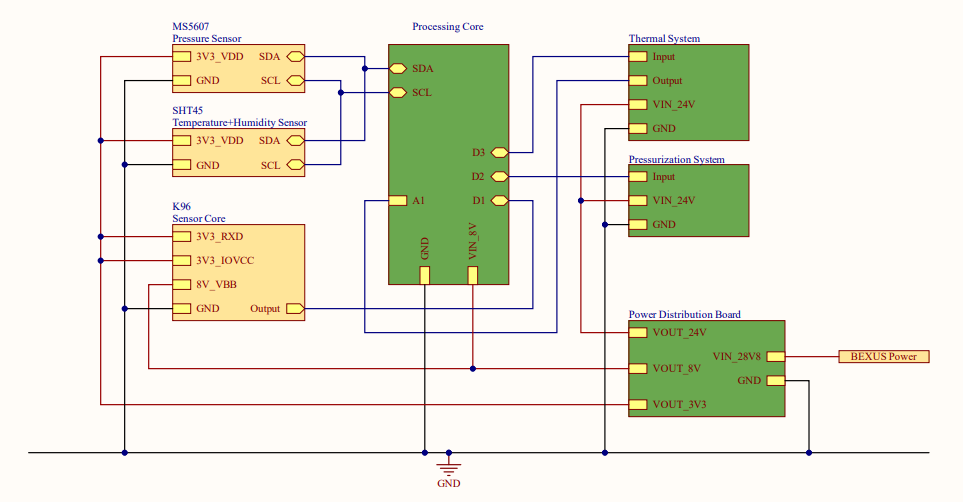
\includegraphics[width=1.0\textwidth]{0_images/figures/Mirage_Electrical_Schematic.png}
            \caption{Electrical Schematic}
                \label{fig:electrical_schematic}
                \end{figure}

\subsection{Processing core unit}

%\begin{figure}[H]
%    \centering
%    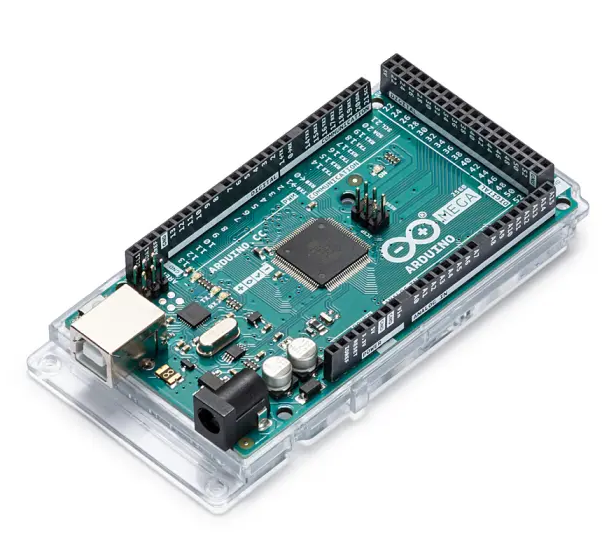
\includegraphics[width=0.5\textwidth]{0_images/figures/Arduino MEGA Rev3.png}
%    \caption{Arduino Mega Rev3 WiFi}
%    \label{fig:component_arduino}
%\end{figure}


An Arduino Mega will be used for preliminary testing and as a backup solution, and will be replaced by a dedicated processing \gls{pcb} once assembly begins. The Arduino Mega is equipped with an Ethernet shield, enabling it to communicate with EGSE and save measurement data to an SD card. The Arduino needs a power input between 7-12V, which will be converted from the 28.8V provided by Bexus' SAFT batteries through a DC/DC stepdown regulator.

\subsection{MicroSD Card}

%\begin{figure}[H]
%    \centering
%    
\includegraphics[width=0.3\textwidth]{0_images/figures/MicroSD card.png}
%    \caption{SDHC Memory Card}
%    \label{fig:component_SDHC}
%\end{figure}

Measurement data will be stored on a microSDHC memory card (SP016GBSTHBU1V10SP) with a capacity of 16~GB. The card has maximum read and write speeds of up to 85~MB/s and 15~MB/s, respectively. The device operates within a supply voltage range of 2.7--3.6~V and an operating temperature range of 0\degree C to 70\degree C.

The card interfaces with the processing core unit via the SPI (Serial Peripheral Interface), using the MOSI, MISO, SCK, and CS signals for data transfer and control.

\subsection{Power Distribution Board}

%\begin{figure}[H]
%    \centering
%    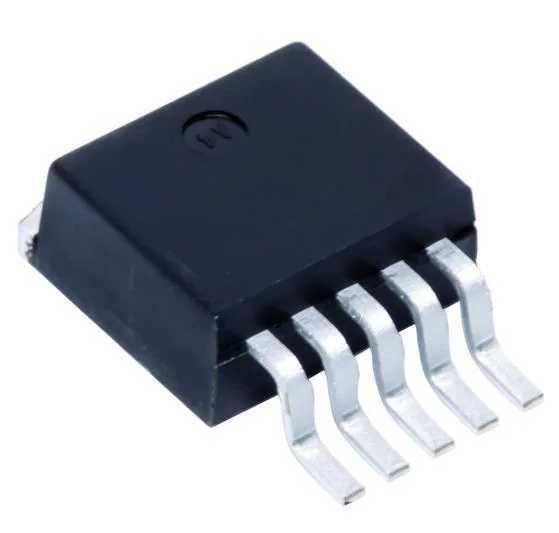
\includegraphics[width=0.3\textwidth]{0_images/figures/Stepdown DCDC.png}
%    \caption{LM2596HVS-ADJ step-down DC/DC regulator}
%    \label{fig:component_LM2596HVS-ADJ_DC/DC_regulator}
%\end{figure}
Power distribution within the experiment is handled by a dedicated Power Distribution Board (PDB). The board receives a nominal input voltage of 28.8 V from the BEXUS power system and distributes regulated voltages to the experiment subsystems.

Voltage regulation is implemented using three LM2596HVS-ADJ step-down DC/DC converters. These regulators operate at a switching frequency of 150 kHz, support input voltages up to 57 V, and provide adjustable output voltages in the range of 1.2–37 V. The converters generate three regulated voltage rails required by the experiment: 24 V for the thermal and pressurization systems (compressor and vacuum pumps), 8 V for the K96 NDIR sensor and the MCU, and 3.3 V for the environmental sensors.

To mitigate switching noise introduced by the DC/DC converters on the shared power lines, an LC filter with a cut-off frequency of approximately 4 kHz is implemented on the power distribution board.

Due to the high startup currents expected from the pressurization system, a pre-charge circuit is implemented on the power distribution board to limit inrush currents during system startup.



\subsection{K96 Sensor}

\begin{figure}[H]
    \centering
    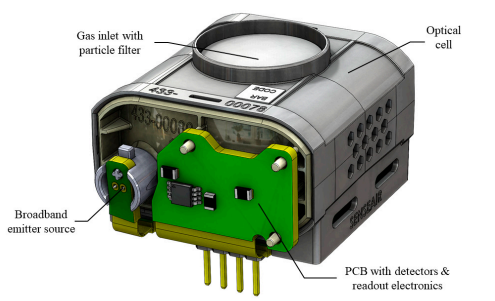
\includegraphics[width=0.5\textwidth]{0_images/figures/K96 Sensor.png}
    \caption{K96 Sensor. Taken from \cite{wastine2022}}
    \label{fig:component_K96_sensor}
\end{figure}

The K96 sensor is a \gls{ndir} gas sensor capable of measuring methane, carbon dioxide, and water vapor. It operates from a 6.0--8.5 V VBB supply and a 2.4--3.6 V IOVCC/RxD logic supply over a temperature range of $-40\degree$C to +85\degree C, with a maximum peak current of 300 mA. The sensor also provides local temperature, pressure, and humidity measurements via an integrated BME280 sensor.

\subsection{Temperature and Humidity Sensor}

%\begin{figure}[H]
%    \centering
%    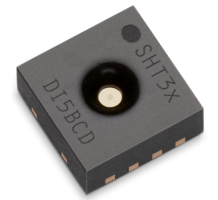
\includegraphics[width=0.3\textwidth]{0_images/figures/Humidity Sensor.png}
%    \caption{SHT3X-DIS Humidity Sensor}
%    \label{fig:component_SHT3X-DIS_humidity}
%\end{figure}

The ambient temperature and humidity sensor is a SHT45, with an operating range of -40 to 125$^\circ$C and a humidity measurement range of 0--100\% RH. The sensor provides a humidity accuracy of $\pm 1.0$ \% RH and a temperature accuracy of $\pm 0.1\,^\circ$C. Communication with the sensor is performed via an I$^2$C digital interface, allowing temperature and humidity data to be read directly by the processing unit. The operating voltage range is 1.08 V to 3.6 V, with a typical average current consumption of approximately 0.4 $\mu$A.

\subsection{Pressure Sensor}
The ambient pressure sensor MS5607 is a barometric sensor that provides a highly linear
and precise 24-bit pressure and temperature value. It has I$^2$C and SPI interface up to
20MHz and has can measure between 10-1200mbar with an accuracy of ±1.5mbar. The
operating temperature range is -40 to 85\degree C and the supply voltage is between 1.8 and
3.6V

\subsection{Pressurization system}
The pressurization system is powered through the experiment power distribution board and controlled by the processing unit. The system includes two diaphragm vacuum pumps and a piston compressor, which together provide the airflow and pressure increase required for the measurement chamber. The system operates at 24 V and is supplied through the experiment power distribution system.

Pressure sensors will be installed between the compression stages and inside the measurement chamber to monitor system performance. These sensors provide feedback to the processing unit, enabling monitoring of the internal pressure and verification of correct system operation.

A passive outlet is used to allow air to exit the measurement chamber. The outlet is implemented as a fixed flow restriction that enables continuous exhaust of air while the pumps and compressor maintain the required chamber pressure. The internal chamber pressure is therefore primarily regulated by the pressurization system, while the passive outlet ensures continuous gas exchange within the chamber.

Detailed electrical interfaces, component specifications, and control parameters will be defined during the detailed design phase following component selection and testing.

%%%%%%%%%%%%%%%%%%%%%%%%%%%%%%%%%%%%%%%%%%%%%%%%%%%%%%%%%%%%%%%%%%%%%%%%%%%%%%%
\section{Thermal Design}\label{sec: thermal design}
\begin{figure}[H]
    \centering
    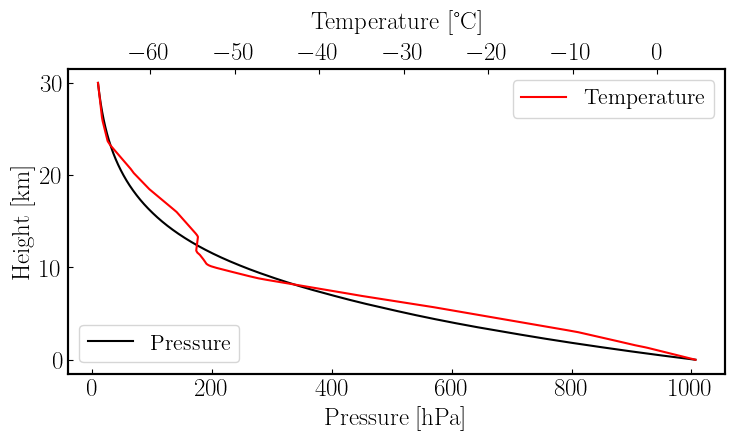
\includegraphics[width=0.8\textwidth]{0_images/figures/pressure_temperature_profile.png}
    \caption{Averaged pressure and temperature profile obtained by the Sodankylä weather station in Finland over all days of October 2025.}
    \label{fig:temp_press_profile}
\end{figure}

The temperature conditions in a stratospheric balloon flight are quite extreme with temperatures reaching as low as -80\degree C. At the same time the air pressure can drop as low as 10 mbar, which also implies that convective heat transfer is very weak, which might cause a poorly designed system to overheat. An averaged ambient pressure and temperature profile is shown in \fref{fig:temp_press_profile}. The low temperatures might cause substantial convective cooling at lower altitudes of around 8 km, while the low pressure in combination with solar radiation might cause substantial internal and radiative heating. 
In the following, the worst hot and cold cases will be analysed, and expected temperatures of the experiment will be shown by referencing the expected pump operations schedule.\par 

\subsection{Thermal analysis background}
A detailed description is given in \aref{app:thermal_background}.


\subsection{Cold case}\label{sec: thermal cold case}
The cold case is a steady state assumption, given environmental conditions at a specific altitude. The appropriate altitude is determined as the maximum of the air heat convection $Q_\mathrm{conv}(h)$ profile from the averaged temperature and pressure profiles given in \fref{fig:temp_press_profile}. It is assumed that no solar radiation is impacting the system (except \gls{ir} radiation from the Earth). Ambient pressure is taken from \fref{fig:temp_press_profile}, while the ambient temperature is set to be $-80$°C. Notably, the tubes containing pressurised, hot air, are assumed to be perfect thermal insulators, which is far from accurate. However, as the heat flux provided by the heated air is very small, this is acceptable.\par 
To estimate impact of different operations and system designs, the analysis takes into account whether pumps are turned on or off, whether the experiment has heaters or not and whether the experiment is insulated or not. The insulation is assumed to be a 5 cm thick box of styrofoam, completely encapsulating the chassis. The pumps are assumed to draw 50 W. This corresponds to the maximum power draw possible by two diaphragm pumps and one piston compressor. The active pumps were chosen according to the operations schedule as outlined in \sref{sec: pump system arch}. Assuming an efficiency of 60\% for the diaphragm pumps and 40\% for the piston compressor, the resulting heat load is 26 W.\par 

In \tref{tab:thermal results cold case} the results of the cold case analysis are displayed. 
Without the styrofoam insulation, the chassis reaches dangerously low temperatures, even with an active heating system. The heating system then would require over 75 W, which is unfeasible. Even with the styrofoam insulation, the required heating power is around 22 W, which is unsustainable for longer periods of time. However, when the pumps are being used, their heat alone is enough to keep the chassis and chamber within desired temperatures. The cold case analysis therefore concludes a necessity of insulation and active pumps.


\begin{table}[H]
\centering
\caption{Thermal Performance Analysis: Cold Case Scenarios at 8.8\,km Altitude}
\label{tab:thermal results cold case}
\begin{tabular}{@{}lll S[table-format=-2.2] S[table-format=-2.2] S[table-format=-2.2]@{}}
\toprule
\textbf{Insulation} & \textbf{Pumps} & \textbf{Thermal System} & {$T_{Chassis}$ [\si{\celsius}]} & {$T_{Chamber}$ [\si{\celsius}]} & {Power [\si{W}]} \\ \midrule
None & Off & None & -79.27 & -79.27 & {---} \\
None & Off & Active & -29.02 & 21.00 & 75.23 \\ 
Styrofoam & Off & Passive & -78.70 & -78.70 & {---} \\
Styrofoam & Off & Active & 6.52 & 21.00 & 21.79 \\ \midrule
None & Active & None & -61.80 & -61.80 & {---} \\
None & Active & Active & -20.40 & 21.00 & 62.28 \\ 
Styrofoam & Active & Passive & -72.41 & -72.41 & {---} \\
Styrofoam & Active & Active & 21.14 & 21.00 & -0.21 \\ \bottomrule
\addlinespace
\multicolumn{6}{l}{\small \textit{Note: Negative power values indicate active cooling required to maintain target temperature.}}
\end{tabular}
\end{table}

\subsection{Hot case}\label{sec: thermal hot case}
Similar to the cold case, the hot case will follow a lumped system approach. However, the appropriate altitude here is chosen to minimize the impact of heat convection via air and maximizing solar heating. This means that the hot case will assume environmental conditions like those found at 30 km altitude, namely $T=-66$°C, $p=0.01$ bar and cloud-free skies. As in the cold case analysis, the effects of pumps, active heating, and styrofoam insulation are tested for individually. The results are displayed in \tref{tab:thermal results hot case}. Without styrofoam insulation, and no thermal system/heating or active pumps, the chassis temperature will reach around $-3$°C. 
Adding the insulation leads to a counterintuitive temperature reduction to $-47$°C. This is due to the styrofoam reflecting more sunlight than the aluminium, while simultaneously loosing heat more efficiently via \gls{ir} radiation. 
As the heat loads involved are comparatively small, an active heating system has to provide around 14 W to raise the chamber temperature to 21°C. However, if pumps are active at 30 km altitude, the chassis will quickly reach temperatures higher than 21°C, requiring cooling of around 9 W instead.\par 

In conclusion, the hot case analysis shows that active pumps at high altitudes will necessitate a cooling system. In order to avoid complexity, it is therefore favourable to avoid using the pumps at high altitudes. 
This agrees well with the planned operations for the pumps, as given in \sref{sec: pump system arch}.

 


\begin{table}[H]
\centering
\caption{Thermal Performance Analysis: Hot Case Scenarios at 30\,km Altitude}
\label{tab:thermal results hot case}
\begin{tabular}{@{}lll S[table-format=-2.2] S[table-format=-2.2] S[table-format=-2.2]@{}}
\toprule
\textbf{Insulation} & \textbf{Pumps} & \textbf{Thermal System} & {$T_{Chassis}$ [\si{\celsius}]} & {$T_{Chamber}$ [\si{\celsius}]} & {Power [\si{W}]} \\ \midrule
None & Off & None & -3.16 & -3.16 & {---} \\
None & Off & Active & 16.39 & 21.00 & 6.93 \\ 
Styrofoam & Off & Passive & -47.32 & -47.32 & {---} \\
Styrofoam & Off & Active & 11.89 & 21.00 & 13.71 \\ \midrule
None & Active & None & 65.10 & 65.10 & {---} \\
None & Active & Active & 30.25 & 21.00 & -13.92 \\ 
Styrofoam & Active & Passive & -29.47 & -29.47 & {---} \\
Styrofoam & Active & Active & 26.75 & 21.00 & -8.65 \\ \bottomrule
\addlinespace
\multicolumn{6}{l}{\small \textit{Note: Negative power values indicate active cooling required to maintain desired chamber temperature.}}
\end{tabular}
\end{table}


\subsection{Continuous operation}
As before, the continous operation usses a lumped system approach. However, now the total energy of the system is not assumed to be constant, but transient. This means that the system temperature is changing with the changing environmental and internal heat loads. Therefore, thermal inertia needs to be taken into account via
\begin{align}
    mc_{p}\dot{T} =& Q_\mathrm{ele}+Q_\mathrm{pump}(h)+Q_\mathrm{transfer} + Q_\mathrm{rad\,in}(h) + Q_\mathrm{insulation} - Q_\mathrm{conv}(h) - Q_\mathrm{rad\,out} \label{eq: heat diff chassis}
\end{align}
for the chassis. As before, the power required to keep the pressure chamber at 21°C can be calculated via \eqref{eq:heat_balance_chamber}, since $\dot{T}$ is supposed to be equal to 0 for the chamber. 
In this scenario the pumps operate by the operating plan specified in \sref{sec: pump system arch}. Additionally, pumps and thermal systems are activated 30 minutes before launch to simulate pre-heating and pre-pressurisation of the chamber. Otherwise the pumps are assumed to work on lower power draw settings at altitudes under 14 km, adding an estimated heat load of 18 W. Between 14 km and 22 km, the pumps operate at full power, adding a heat load of 26 W. Beyond 22 km the pumps are switched off. The total flight time is estimated to be 6 h long. 
The float phase is assumed to be at constant 26 km altitude. The heating system is assumed to be capable of a maximum heating output of 10 W.
After the pumps are deactivated at 22 km, the heating system aims to stabilise the chamber temperature at $-5$°C. This is done as a proxy to prevent the electronics in the chassis from freezing.\par 

The result for an experiment inside a styrofoam insulation box and subject to solar daylight is shown in \fref{fig:continous thermal sim main}. 
%As expected, heating is especially necessary between ca 8 km and 14 km. 
The chassis temperature never drops much below $-10$°C, while the thermal power requirements do not reach the set maximum of 10 W.  
By integrating the power requirement curve one obtains a total required heating power of $\approx 29.45$ Wh. This result refers to heating energy and not to the energy necessary to power heating components, which is expected to be greater.\par 
If no insulation were used, the total required heating power would jump to 37.45 Wh. If insulation were used, but no daylight were available, the heating power required would be 36.42 Wh. The temperature and heating curves for both cases are provided in \fref{fig:continous thermal sim side}. If no insulation is used, the heating system is unable to keep the chamber temperature within the required temperature range of 15°C to 40°C during ascend. It also fails at keeping the chassis temperature within a safe range of -15 to 65°C during descend. On the other hand, if insulation is used, but the flight is during night time or particularly cloudy conditions, the effects are rather minimal. The heater would max out its power output and the chassis temperature would drop to around $-15$°C during descend, which is just the lower limit of the safe range and still 10°C away from the strict lower limit of -25°C.

\begin{figure}[htbp]
    \centering
    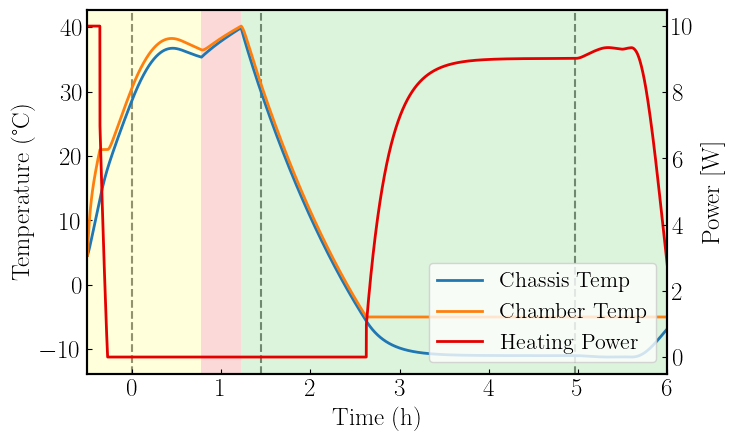
\includegraphics[width=0.8\textwidth]{0_images/figures/thermal_analysis_plot_WITHins_WITHlight.png}
    \caption{Expected temperature of the chassis and chamber and the heating power necessary to sustain 21°C in the chamber. The gray lines indicate the time intervals when the balloon is ascending, floating, and descending. The colors indicate different power settings of the pressurisation system: green - no pumps, yellow - low power, red - high power.}
    \label{fig:continous thermal sim main}
\end{figure}

\begin{figure}[htbp]
\begin{subfigure}[c]{0.5\linewidth}
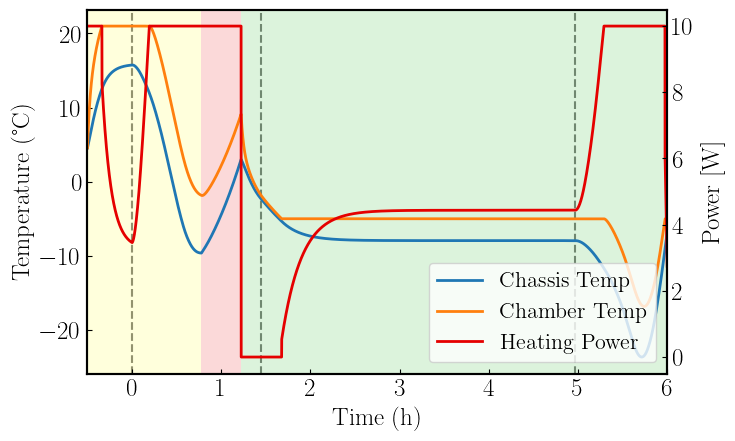
\includegraphics[width=\linewidth]{0_images/figures/thermal_analysis_plot_NOins_WITHlight.png}
\caption{No insulation, with daylight.}
\end{subfigure}
\hfill
\begin{subfigure}[c]{0.5\linewidth}
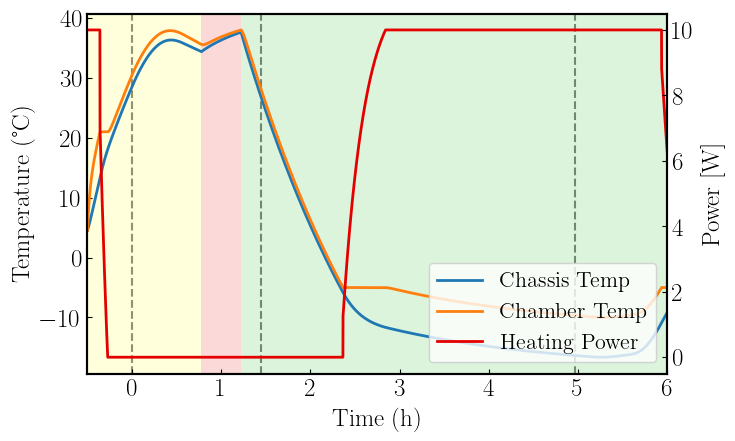
\includegraphics[width=\linewidth]{0_images/figures/thermal_analysis_plot_WITHins_NOlight.png}
\caption{With insulation, no daylight}
\end{subfigure}%
\caption{Expected temperature of the chassis and chamber and the heating power necessary to sustain 21°C in the chamber. The gray lines indicate the time intervals when the balloon is ascending, floating, and descending. The colors indicate different power settings of the pressurisation system: green - no pumps, yellow - low power, red - high power.}
\label{fig:continous thermal sim side}
\end{figure}

\subsection{Conclusion}\label{sec: thermal conclusion}
The cold and hot case analysis shows that the experiment if enclosed in a styrofoam insulation is able to stay within the required temperature range depending on the proper use of pumps. In the ascend phase, the pumps are generating enough heat to keep the chamber temperature at 21°C, even without additional heating elements. In fact the transientt analysis shows that temperatures of chassis and chamber might reach close to 40°C. During float phase, the chamber temperature is allowed to drop to $-5$°C. This is done in order to keep the electrical components within the chassis at around $-10$°C. The required total heating power for daytime and nighttime would be $\approx 29.45$ Wh and $\approx 36.42$ Wh, respectively. Depending on the final design of the electrical components, the temperature limit and thus required power might be lowered further.

\subsection{Passive thermal control system}
The above analysis shows that white styrofoam is a good candidate for insulation. The chassis is planned to be completely sourrounded by 5 cm thick styrofoam insulation. Further analysis on other insulation materials and implementations, as well as on other passive control systems, will commence with the start of thesis project 6 and 7 (see \tref{tab:thesis}). Additionally, the intake air will be preheated before being fed to the diaphragm pumps. This can be done via a thermally conductive, solenoid shaped tubing housed inside the chassis. If the tubing has higher heat capacity than the incoming air, it can act as a heat sink, heating the incoming air to an acceptable temperature. The exact shape and length of the tube will be determined via tests.

\subsection{Active thermal control system}
The above analysis shows that during ascend and before launch, the pumps alone will provide enough heating power to heat the chamber to around 40°C. This is on the edge of the acceptable temperature range as outlined in \tref{tab:design_req}, P.7. Further analysis of overheating mitigation methods, including pump duty cycles and other active thermal control methods will commence with the start of thesis project 6 (see \tref{tab:thesis}).\par 

During float and descend, the above analysis shows that a 10 W heater is sufficient to keep the electronics inside the chassis within acceptable limits, see \tref{tab:design_req}, D.1.3. There are multiple common choices for thermal control components at low wattages and high precision. These will be discussed below.
\paragraph{\gls{ptc} ceramics} are commonly used in portable space heaters. They are used via resistive heating. However, due to their \gls{ptc}, a rising internal temperature causes their resistivity to increase as well. This behaviour can be configured, such that a desired maximum temperature can be set at which the ceramic resistivity becomes too high for the temperature to rise further. They are therefore self regulating, adding additional security and requiring less controlling. They are also quite cheap. However, because they are made of ceramic, they can not easily fit inside a tight experiment. 

\paragraph{Peltier devices} are heat pumps, that transfer heat from one side of the device to the other when an electrical current is applied. Upon reversal of the current polarity, the heat transfer flow is also reversed. These devices can therefore be used to cool and heat. This makes them great candidates for an active thermal control system that has to cool and heat components depending on mission phase. The downside is that they require heat sinks that the excess heat (or lack thereof) can be dumped to. They also require more sophisticated controlling software and circuits to be able to switch between cooling and heating.

\paragraph{Polyimide film heating elements} consist of a thin conductive heating element sourrounded by polyimide film. They are very flexible, sturdy and commonly used in space environment heating solutions. Although they are not self regulating, they can be easily controlled using \gls{pid} algorithms. They are unable to provide cooling, but offer a great surface area to enable uniform heating. Due to their flexibility, they are also easy to integrate into a system and do not require complex software or circuits.\par  

Because of the low heating power required, the small operating temperature expected, the ease of integration, its big surface area, and its low cost a polyimide film heating element is chosen. The heating element is included in \tref{tab:power_consumption}. It can be attached via \gls{psa} and wrapped around the pressure chamber. Since the chamber is made out of aluminium, and aluminium is good thermal conductor, one heating pad should suffice. This will be confirmed by tests. Should tests show that there is indeed no need for heating the pressurisation chamber, the heater may be moved directly to the temperature sensitive electrical components like the \gls{pcb}.\par 

The heating pad will be controlled using a \gls{pid} algorithm, as common for heating appliances. The algorithm will run on the \gls{mcu}. The \gls{mcu} then controls the heating power of the heating pad by adjusting its duty cycle by powering a \gls{mosfet}. The exact \gls{pwm} setting is to be determined by the final \gls{mcu} design. To prevent overheating of the chamber, a \gls{tco} unit is used, wired in series with the heating pad. It can be directly attached via \gls{psa} to the outside of the pressure chamber, monitoring its temperature and breaking the circuit when its temperature reaches above 50°C.


% This can lead to overheating of the electrical components if the heat from dissipated power accumulates. Therefore, it is essential to know how much power is dissipated and to take additional cooling measures in case that radiative cooling is insufficient.

% \begin{table}[H]
% \centering
% \caption{Component Temperature and Power Ratings}
% \label{tab:component_specs}
% \begin{tabular}{p{4cm}p{1cm}p{1cm}p{1cm}p{1cm}p{1cm}p{1cm}}
% \toprule
% \textbf{Component} &
% \multicolumn{2}{c}{\makecell[c]{Operating T (°C)}} &
% \multicolumn{2}{c}{\makecell[c]{Survivable T (°C)}} &
% \multicolumn{2}{c}{\makecell[c]{Power Dissipated (W)}} \\
% \cmidrule(lr){2-3} \cmidrule(lr){4-5} \cmidrule(lr){6-7}
% & Min & Max & Min & Max & Mean & Max \\
% \midrule
% Pump &  &  &  &  &  &    \\
% Valve &  &  &  &  &  &    \\
% Arduino Mega & -40 & 85 &  &  &  &  1.95  \\
% Switching Regulator & -40 & 125 &  &  &  & 39   \\
% SD Card & -25 & 85 &  &  &  &    \\
% K96 sensor (\gls{ndir}) & 0 & 40 & -40 & 85 &  & 2.447   \\
% BME sensor & -40 & 85 &  &  &  & 0.001   \\
% MS5607 (P) & -40 & 85 &  &  &  & 0.00004   \\
% DS18B20 (T) & -55 & 125 &  &  &  &    \\
% SHT3X-DIS (RH) & -40 & 125 &  &  &  &    \\
% \bottomrule
% \end{tabular}
% \end{table}

% The experiment can be thermally divided into three parts. The coldest part are the ambient sensors on the outside of the experiment box. They are and should be completely exposed and therefore are required to withstand temperatures as low as -80\degree C. This poses a challenge since most commercially available components are made for ground level conditions and manufacturers usually draw the line at -40\degree C for the temperature conditions. If we should get access to a thermal chamber, we can test the reliability of those sensors ourselves at lower temperatures. Since we haven't found sensors with operating ranges going down as low as -80\degree C we might have to resort to this attempt. Those sensors are not central to our experiment. The second part is the electronics compartment, which will likely be not actively heated. The bigger issue for this part might be overheating instead and a careful thermal analysis during the design process will be required to decide on mitigation steps if the temperature ranges of the components are exceeded at the upper or possibly still lower bounds. Later, in the integration process, further tests will follow to verify the functionality of that part at high altitudes.

% The last part is the measurement chamber of which the temperature needs to be more carefully regulated to ensure that the K96 \gls{ndir} sensor, which is central to our experiment, functions properly. Temperature fluctuations can also lead to output drift and therefore we need to keep the temperature in a narrow range. At the same time, pumps, valves or inlet and outlet tube openings could freeze over if the humidity level is high. Since we might fly through clouds with very high humidity levels it is essential that the relative humidity doesn't get too high. By increasing the temperature of the air, condensation can be mitigated and freezing of pumps, valves and tubes should be prevented as well. Further tests will be conducted in later stages of experiment integration.

% Insulation will play another essential role in the thermal design. The whole experiment should be as much thermally separated from the rest of the vehicle as possible. On one hand, this avoids further cooling of the experiment and on the other it avoids impacting other experiment or the vehicle. The measurement chamber should be well insulated as well to not (further) heat up the electronics compartment and to avoid condensation of water on the walls of the chamber.

%%%%%%%%%%%%%%%%%%%%%%%%%%%%%%%%%%%%%%%%%%%%%%%%%%%%%%%%%%%%%%%%%%%%%%%%%%%%%%%
\section{Power design}

The \gls{mirage} team expects to rely exclusively on the 28.8V SAFT MP176065 which is provided by the gondola.

The experiment will have an estimated average current of 0.80A and use 138.67Wh in total, see table 4.9, including the thermal system and the pressurization system. This is higher than previous estimations, mainly due to the thermal system, compressor and vacuum pumps, but this calculation is based on full capacity so it's expected to be lower than this. The peak current draw is high at 2.26A from the BEXUS side for ~30 minutes, see table 4.8, while the compressor and vacuum pumps are working at full capacity, which is close to the requirement D.11.1. 
Since the MCU PCB will be designed by thesis students it is difficult to estimate precisely the current draw for this component, however it was estimated to be 300mA. The K96 has a max current of 300mA but the expected average is lower depending on the time per measurement. 

Before launch, the pressurization system, e.g. vacuum pumps and compressor currents will be limited using some sort of pre-charge circuit and will thus not have a major impact on the energy consumption as a whole. During the flight phase, the pressurization system will be activated in lesser capacity for $\approx 45$ minutes and in full capacity $\approx 30$ minutes in order to conserve energy for the rest of the experiment. After the measurement phase the pressurization system will be limited or completely shut off.

The thermal system will not be activated while the pressurization system is active in order to not exceed current draw limitations and thus will only be operational as detailed in thermal design section.

\begin{table}[H]
\centering
\caption{Max current consumption}
\label{tab:current_consumption}
\begin{tabular}{llllll}
\toprule
\textbf{Amount} & \textbf{Components}& \textbf{Voltage} & \textbf{Current} &\textbf{Power} &\textbf{Energy}\\
\midrule
1 & MCU & 8V & 300mA & 2.4W & 1.2Wh\\
1 & K96 & 8V & 300mA & 2.4 & 1.2Wh \\
2 & MS5607 & 3.3V& 1µA & 6.6µW & 3.3µWh \\
6 & SHT45 & 3.3V & 0.4µA & 7.92µW & 3.96µWh \\
1 & Compressor & 24V & 1.25A & 30W & 15Wh \\
2 & Vacuum pumps & 24V & 0.42A & 20W & 10Wh\\
1 & SDHC & 3.3V & 150 mA & 0.495W & 0.248Wh \\
\midrule
Total &&& 2.45A & 55.295W & 27.648Wh\\
Total (BEXUS) &&28.8V& 2.26A & 65.05W & 32.526Wh \\
\bottomrule
\end{tabular}
\end{table}

\begin{table}[H]
\centering
\caption{Power consumption from the power distribution board and the Bexus power unit}
\label{tab:power_consumption}
\begin{tabular}{L{1.6cm}llllll}
\toprule
\textbf{Duration} & \textbf{Amount} & \textbf{Component} & \textbf{Voltage} & \textbf{Current} & \textbf{Power} & \textbf{Total Energy} \\
\midrule
6h & 1 & MCU & 8V & 300mA & 2.4 W & 14.4Wh \\
1.25h & 1 & K96 & 8V & 300mA & 2.4 W & 3Wh \\
6h & 6 & SHT45 & 3.3 V & 0.4µA & 1.32 µW & 47.52µWh \\
1.25h & 1 & Compressor & 24V & 1.25A & 30W & 37.5Wh \\
1.25h & 2 & Vacuum Pump & 24V & 0.42A & 10W & 25Wh \\
6h & 2 & Pressure sensor & 3.3V & 1µA & 3.3µW & 39.6µWh \\
6h & 1 &SDHC &3.3V& 150mA & 0.495W & 2.97Wh \\
3.5h & 1 &Heating element &12V& 0.83A & 10W & 35Wh \\

\midrule
Average (Bexus) & & & 28.8V & 0.80A & 23.11W\\
Total Bexus Power & & & & & & 138.67Wh \\
\bottomrule
\end{tabular}
\end{table}

Table 4.9 presents key components, amount of components, duration of use, voltage levels, currents and power. The table is representing from the experimenters perspective while the average and total BEXUS power is from the BEXUS power unit perspective. This calculations used the assumption of $85\%$ efficiency to calculate the power consumtion on the BEXUS power unit. 
%%%%%%%%%%%%%%%%%%%%%%%%%%%%%%%%%%%%%%%%%%%%%%%%%%%%%%%%%%%%%%%%%%%%%%%%%%%%%%%
\section{Software design}

The on-board software is responsible for collecting data from the sensors and store it on the on-board SD card. It is also responsible for handling communication from and to ground, as well as the control of the internal pressure and thermal systems and preventing condensation.

For the pressurisation system the software needs to be able to read out the pressure sensor in the measurement chamber and adjust the power of the pumps accordingly to maintain a constant pressure of 3 bar. The mechanical side of the system is explained above. Since the vacuum pumps prepressurise the air that is then compressed to 3 bar, the power of the vacuum pumps and the compressor need to be handled separately. Depending on whether the compressor needs to have a minimum flowrate to work, it might be possible that a pulsed operation is necessary for the compressor, which would put strain on the electrical system. The software needs to be able to adjust these different components accordingly based on the internal pressure sensor. \\

For the thermal control system the software needs to take sensor inputs from different places. It should be split into two different programs, where one is responsible for stabilizing the temperature in the measurement chamber at around room temperature. This also includes controlling potential active heating elements at the gas inlet of the outer enclosure and before the air at 3 bar enters the measurement chamber based on at least on the thermal sensor of the K96 but possibly also several thermal sensor in between. The other thermal control loop should monitor components that are at risk of overheating and components that could underheat. There might be also active heating elements at critical components like the MCU, which could be switched on if the temperatures drop dangerously low inside the electrical compartment. This control loop need to take the different temperature outputs of sensors that are close to the pumps and electrical components and if necessary take counter measures via controlling the heating elements or reducing the power of the pumps.\\
For humidity the role of the software is to detect to high humidity levels (>80\% r.H.). If the ambient sensors detect high levels of humidity outside the software should close the shutter and stop the pumps as a first step to prevent more air with high humidity levels from entering the measurement chamber without losing pressure. When the humidity levels are low enough, the temperature of the air taken into the measurement chamber should be increased slightly by increasing the temperature of the active heating elements until the internal humidity is lower as well.\\


The settings of those systems depend on the readings of the internal and external pressure and temperature sensors. Additionally, correct flight phases need to be engaged. This is done based on longer term changes in the recorded ambient pressure or via a command from the ground, with the command taking priority. A control flow and state diagram are provided in Figure \ref{fig:cont_flow} and Figure \ref{fig:state_diagram}.

The experiment will run on 2 main modes: Manual and Autonomous. Each of the main modes has a submode for standby and active measurements. When the experiment reaches the point where no more data needs to be collected, the system will move to standby mode unless a command has been given to do otherwise. The modes will also allow for autonomous work even through radio blackouts and loss of communication. If below 22\,km and a loss of connection occurs, the system will automatically switch to autonomous measurements mode; if however the experiment is above 22\,km and a loss of connection occurs then the system will switch to Autonomous standby mode that will ensure the experiment remains safe without exhausting any of the hardware.

To guarantee operations watchdog systems will be used to reset the operations if it encountered a fatal error.
The software system will work with different threads working asynchronously.
Data transfer between the threads will happen through producer-consumer queues that are thread-safe.
There will be a thread for reading sensor data, a thread of controlling hardware, a thread sending downlink packages and receiving packages from uplink, a thread to write data on the SD card and finally a thread to control everything with the aid of a watchdog.

All transmissions are saved to the on-board storage with timestamps. Similarly, all saved data is saved with timestamps, too. A table detailing the expected data sizes of data to be stored is given in Table \ref{tab:data_rates}. In total 39856 bits per second (40 kbit) will be stored. This means that for the duration of 6 hours a storage of 108 MB (megabyte) is required to store all the data received from the sensors. The SD cards onboard are more than enough for this task. Some of this data will be downlinked every seconds for redundancy and tracking of the functionality of the experiment. Based on the sampling rates in Table \ref{tab:data_rates},the Elink thread can pull 100 datapoints from the telemetry and data queue to downlink each second, resulting in an estimated downlink rate of 32.8 kbps, below the experiment requirements (P.18) of 100 kbps. Assuming a maximum connection dropout duration of 10 minutes, this would likewise imply a build-up of data of 19.68 Mbit. Transferring it over the next 5 minutes gives a data rate of 65.6 kbps which is feasible. With compression it is probable that only half the rates stated need to be transmitted, but a higher data rate could be used to send duplicates or checksums for error mitigation.

The frequencies are chosen based on the datasheets of the sensors. The SHT45 sensor has multiple modes, fast mode plus (FM+) was chosen for this mission. The K96 sensor relies on the speed of the NDIR sensor within with typically is below 10 Hz, whereas in the MS5607 sensor OSR 4096 mode was chosen. The \gls{rtc} frequency was calculated to be equal to all the frequencies added. This is to consider the scenario where none of the sensors data readings collide and all the readings from the 3 sensors are collected at different timestamps, which will require one timestamp for each.

The K96 sensor core requires a UART interface and relies on the Modbus protocol, while most other sensors use I2C. The communication protocol will be UDP.

\begin{table}[H]
\centering
\caption{Max sampling rates, sampling sizes, and data rates of data products to be stored}
\label{tab:data_rates}
\begin{tabular}{p{7cm}p{2cm}p{2cm}p{2cm}}
\toprule
\textbf{Component} & \textbf{Max. sampling rate [Hz]} & \textbf{Sampling size [bit], includes CRC} & \textbf{Data rate [bps]} \\
\midrule
LPL (K96) & 10 & 32 & 320\\
SPL (K96) & 10 & 32 & 320\\
MPL (K96) & 10 & 32 & 320\\
Pressure (K96) & 10 & 16 & 160\\
Temperature (K96) & 10 & 16 & 160\\
Relative Humidity (K96) & 10 & 16 & 160\\
Internal pressure sensor (MS5607) & 110 & 28 & 3080 \\
Internal temperature sensor (SHT45) & 222 & 24 & 5328 \\
Internal humidity sensor (SHT45) & 222 & 24 & 5328 \\
Ambient pressure sensor (MS5607) & 110 & 28 & 3080 \\
Ambient temperature sensor (SHT45) & 222 & 24 & 5328 \\
Ambient humidity sensor (SHT45) & 222 & 24 & 5328 \\
Real Time Clock & 342 & 32 & 10944\\
% \dos{General housekeeping data} (current for e.g. pumps, data from thermal system, ...) & 1 & 384 & 384 \\
\midrule
Total & & & 39856 \\
\bottomrule
\end{tabular}
\end{table}

\begin{figure}[H]
\centering
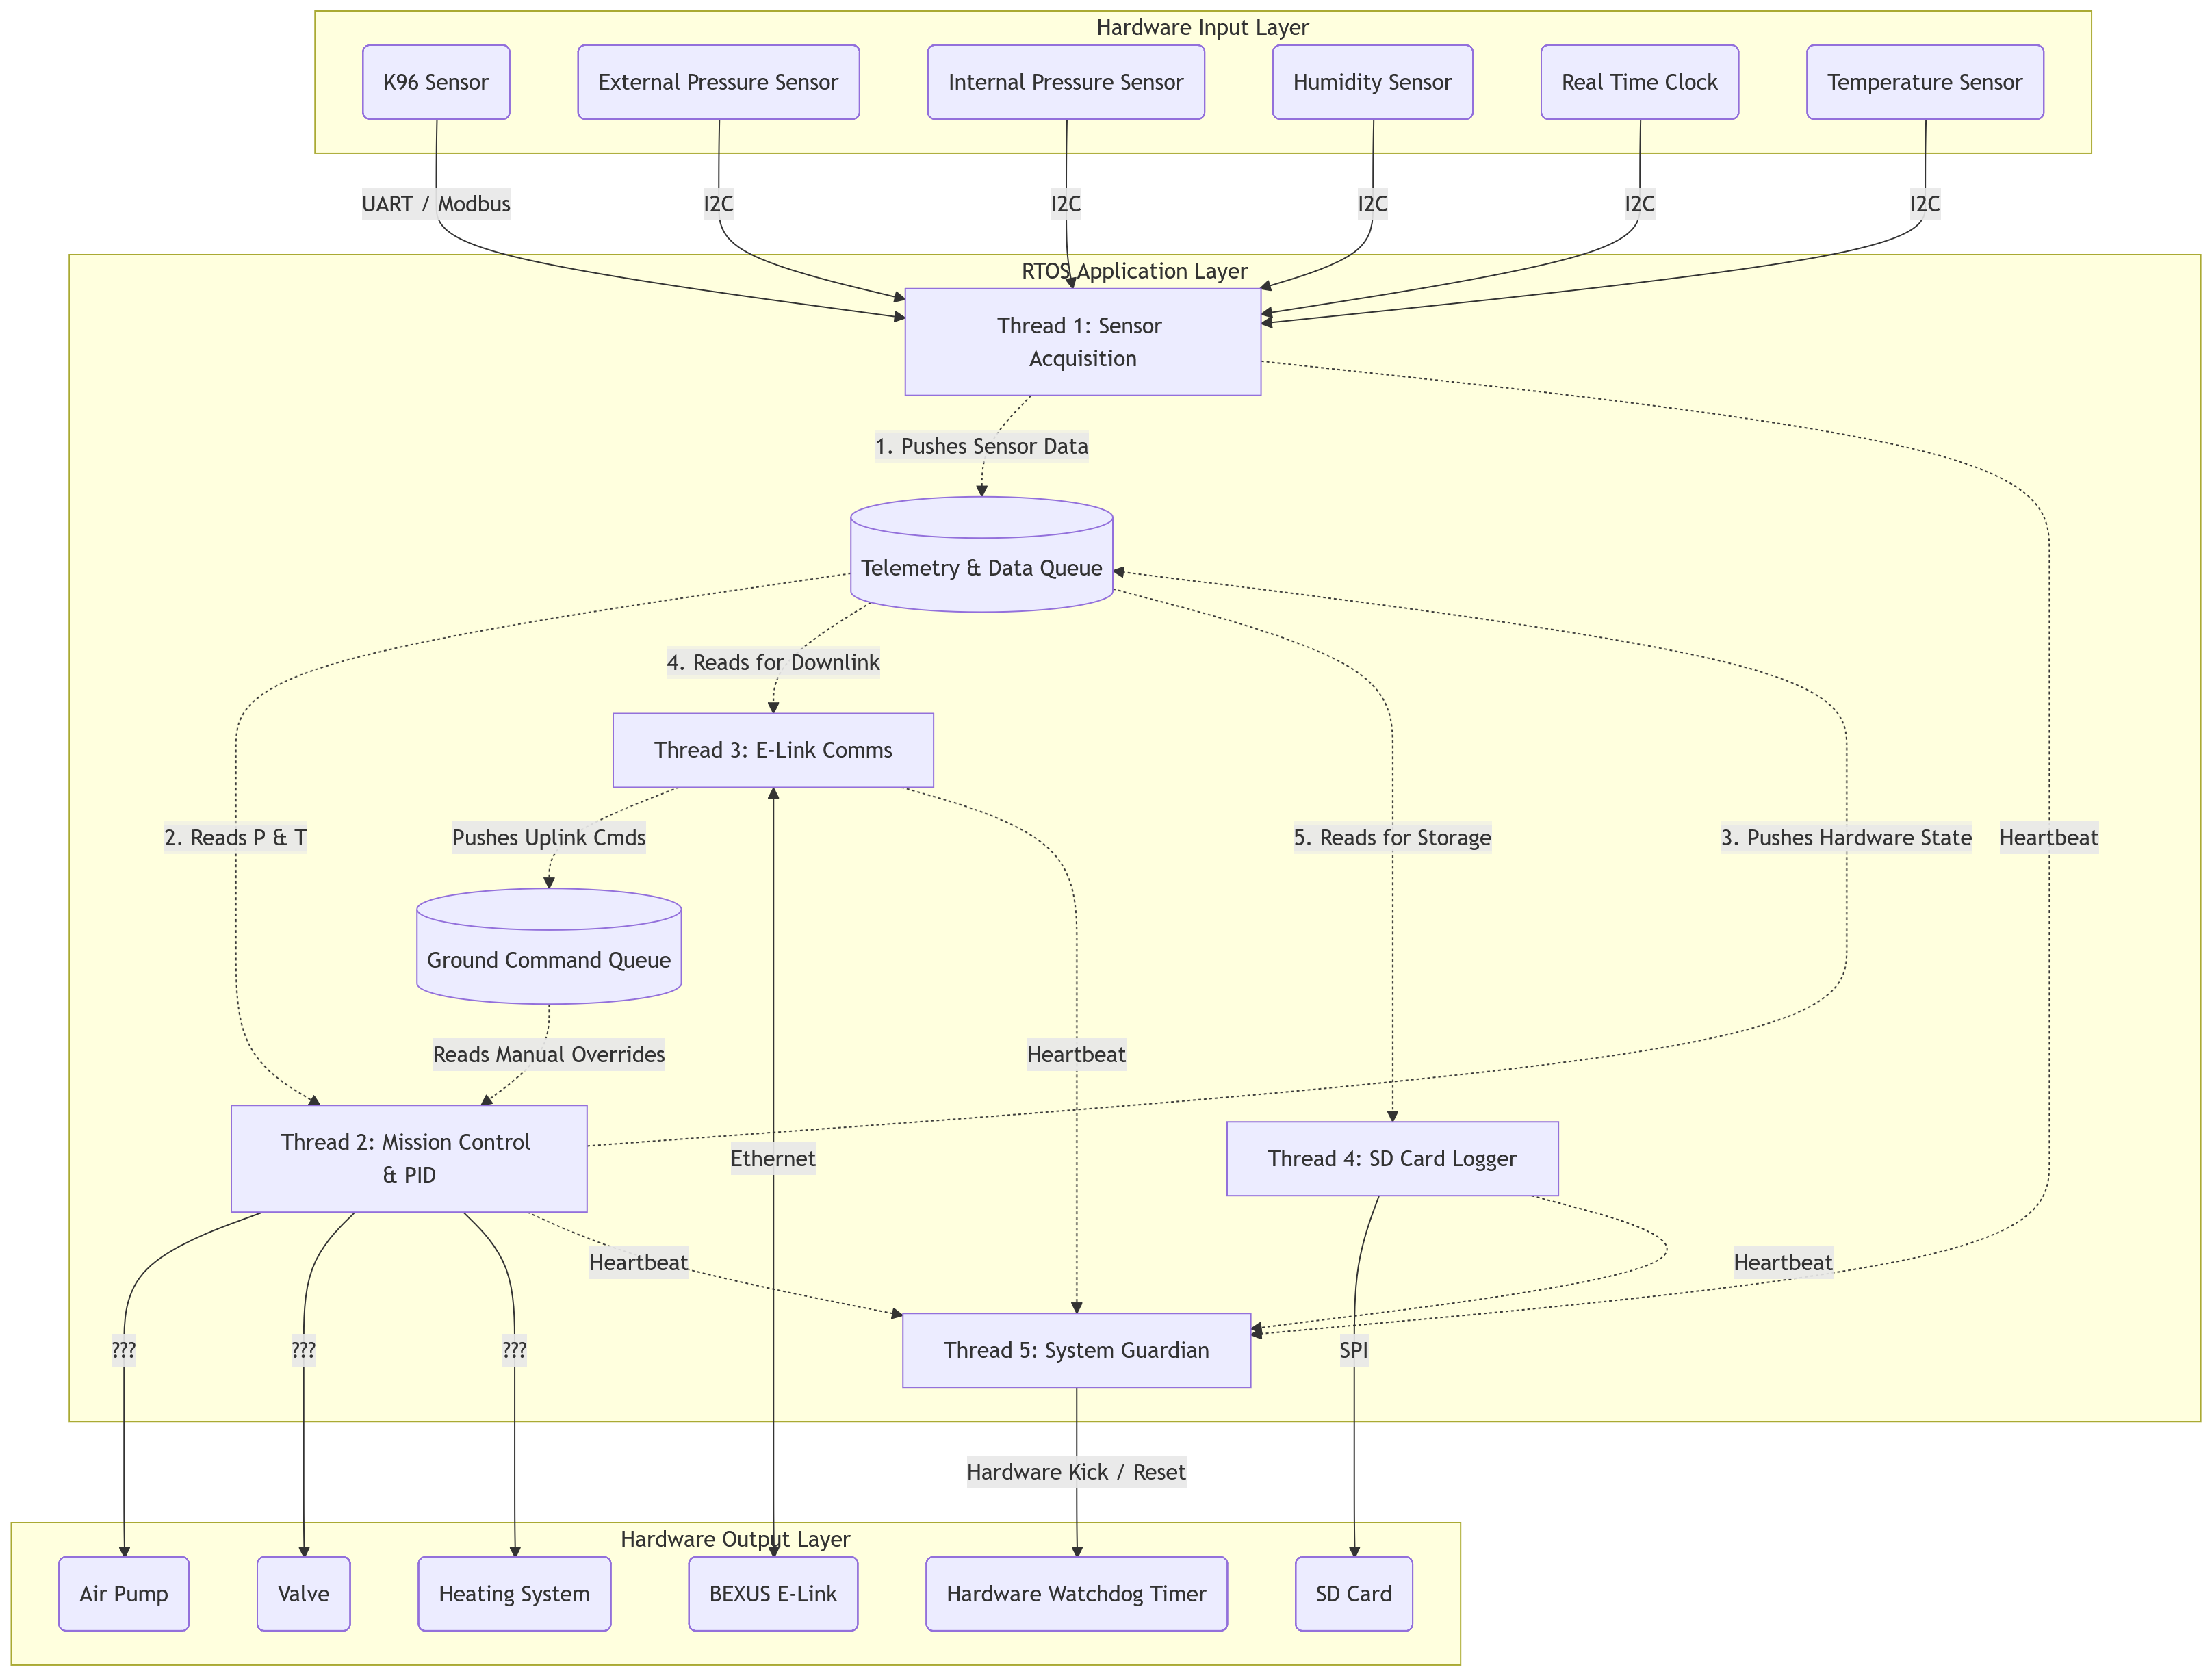
\includegraphics[width=.9\textwidth]{0_images/figures/control_flow.png}
\caption{Control flow diagram}
\label{fig:cont_flow}
\end{figure}

\begin{figure}[H]
\centering
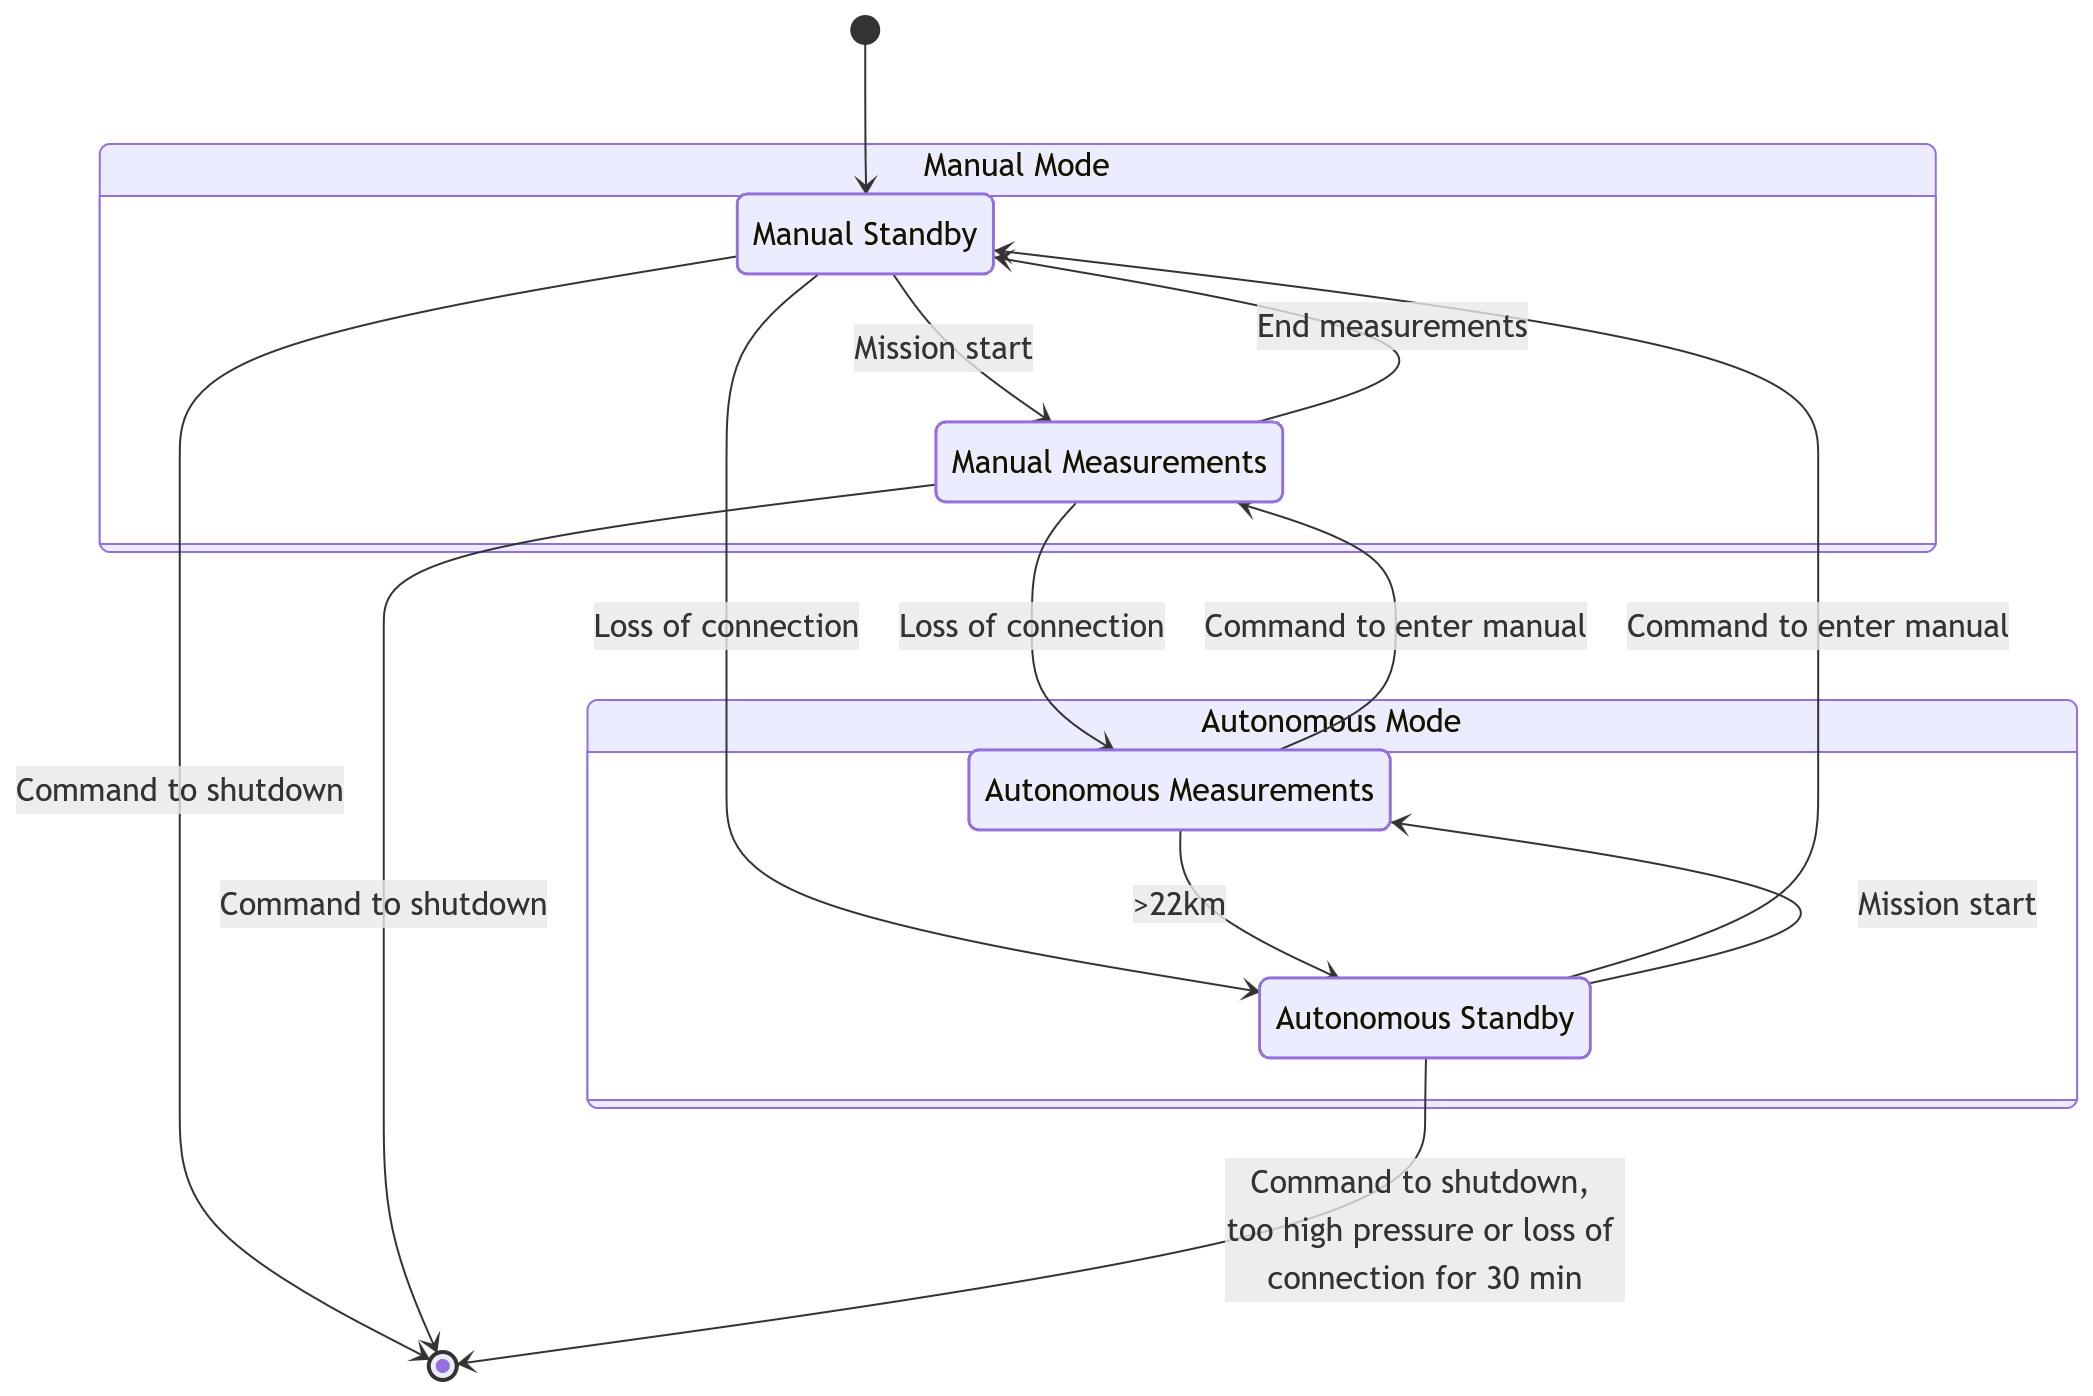
\includegraphics[width=\textwidth]{0_images/figures/state_chart.png}
\caption{State diagram}
\label{fig:state_diagram}
\end{figure}

%%%%%%%%%%%%%%%%%%%%%%%%%%%%%%%%%%%%%%%%%%%%%%%%%%%%%%%%%%%%%%%%%%%%%%%%%%%%%%%
\section{Ground support equipment}

A Python-based \gls{gui} will be developed for ground operations during the mission. The interface will be implemented using a suitable graphical library such as Tkinter, PyQt, or PySide, depending on the final balance between simplicity, responsiveness, and development effort. For plotting and visualizing received downlink data, libraries such as Matplotlib or PyQtGraph can be used, while the downlink data itself will also be stored locally on the ground computer for later inspection and post-flight analysis.

The \gls{gui} will include clickable buttons for common mission commands, allowing operators to send predefined instructions through uplink without manually typing them each time. In addition, the interface will contain a terminal section for commands or configuration options that are not part of the predefined buttons, providing flexibility for debugging, manual intervention, and ad-hoc control during operations.

Additionally the team will require basic electronic equipment, chairs and a table to operate from and troubleshoot any issues before flight.

%%%%%%%%%%%%%%%%%%%%%%%%%%%%%%%%%%%%%%%%%%%%%%%%%%%%%%%%%%%%%%%%%%%%%%%%%%%%%%%